%%%%%%%%%%%%%%%%%%%%%%%%%%%%% Thesis.tex %%%%%%%%%%%%%%%%%%%%%%%%%%%%%%%
%                                                                      %
%  ---------- Master of Science Dissertation template ----------       %
%                                                                      %
%  Template for the Master Thesis according to the regulations         %
%  published by the Academic Board (Direcção Académica) at IST.        %
%                                                                      %
%  For up-to-date guide, please refer to the official website          %
%  http://academica.tecnico.ulisboa.pt/alunos/dissertacao-de-mestrado/ %
%                                                                      %
%       Andre C. Marta                                                 %
%       Area Cientifica de Mecanica Aplicada e Aeroespacial            %
%       Departamento de Engenharia Mecanica                            %
%       Instituto Superior Tecnico                                     %
%       Av. Rovisco Pais                                               %
%       1049-001 Lisboa                                                %
%       Portugal                                                       %
%       Tel: +351 21 841 9469                                          %
%                        3469 (extension)                              %
%       Email: andre.marta@tecnico.ulisboa.pt                          %
%                                                                      %
%  Created:       Jan 20, 2011                                         %
%  Last Modified: Feb 19, 2018                                         %
%                                                                      %
%%%%%%%%%%%%%%%%%%%%%%%%%%%%%%%%%%%%%%%%%%%%%%%%%%%%%%%%%%%%%%%%%%%%%%%%
%  Revision history                                                    %
%  v1 - 2011/01/24 - original template                                 %
%  v2 - 2012/10/30 - new IST image and glossary support                %
%  v3 - 2013/12/10 - update according to 2012/13 official guide        %
%  v4 - 2014/02/28 - new default for bibliography style                %
%  v5 - 2014/05/07 - update according to 2013/14 official guide        %
%  v6 - 2015/07/02 - cover page format fixed,                          %
%                    contents page numbering fixed,                    %
%                    better language support,                          %
%                    enhanced examples of tables,                      %
%                    new option for appendix page numbering format,    %
%                    custom bibliography style                         %
%  v7 - 2018/02/19 - multiple citations compressed                     %
%%%%%%%%%%%%%%%%%%%%%%%%%%%%%%%%%%%%%%%%%%%%%%%%%%%%%%%%%%%%%%%%%%%%%%%%
%                                                                      %
% To generate the PDF file, type "make" at the terminal prompt.        %
%                                                                      %
% The IST template LaTeX package was created by the author             %
% and it can be downloaded from:                                       %
% https://fenix.ist.utl.pt/homepage/ist31052/                          %
%                                                                      %
% The external packages can be downloaded from                         %
% the Comprehensive TeX Archive Network at http://www.ctan.org/        %
%                                                                      %
% List of LaTex symbols:                                               %
% http://www.ctan.org/tex-archive/info/symbols/comprehensive/          %
%                                                                      %
% Help with LaTex can be found at                                      %
% http://www.giss.nasa.gov/tools/latex/ltx-2.html                      %
% http://en.wikibooks.org/wiki/LaTeX                                   %
%%%%%%%%%%%%%%%%%%%%%%%%%%%%%%%%%%%%%%%%%%%%%%%%%%%%%%%%%%%%%%%%%%%%%%%%

%%%%%%%%%%%%%%%%%%%%%%%%%%%%%%%%%%%%%%%%%%%%%%%%%%%%%%%%%%%%%%%%%%%%%%%%
%     Preamble                                                         %
%%%%%%%%%%%%%%%%%%%%%%%%%%%%%%%%%%%%%%%%%%%%%%%%%%%%%%%%%%%%%%%%%%%%%%%%

% ----------------------------------------------------------------------
%  Set the document class
% ----------------------------------------------------------------------
\documentclass[10pt,a4paper,twoside]{report}

% ----------------------------------------------------------------------
% Define external packages, language, margins, fonts and new commands
% ----------------------------------------------------------------------
%%%%%%%%%%%%%%%%%%%%%%%%%%%%%%%%%%%%%%%%%%%%%%%%%%%%%%%%%%%%%%%%%%%%%%%%
%                                                                      %
%     File: Thesis_Preamble.tex                                        %
%     Tex Master: Thesis.tex                                           %
%                                                                      %
%     Author: Andre C. Marta                                           %
%     Last modified : 9 Apr 2015                                       %
%                                                                      %
%%%%%%%%%%%%%%%%%%%%%%%%%%%%%%%%%%%%%%%%%%%%%%%%%%%%%%%%%%%%%%%%%%%%%%%%

% ----------------------------------------------------------------------
% Define document language.
% ----------------------------------------------------------------------

% 'inputenc' package
%
% Accept different input encodings.
% http://www.ctan.org/tex-archive/macros/latex/base/
%
% > allows typing non-english text in LaTeX sources.
%
% ******************************* SELECT *******************************
%\usepackage[latin1]{inputenc} % <<<<< Windows
\usepackage[utf8]{inputenc}   % <<<<< Linux
% ******************************* SELECT *******************************


% 'babel' package
%
% Multilingual support for Plain TeX or LaTeX.
% http://www.ctan.org/tex-archive/macros/latex/required/babel/
%
% > sets the variable names according to the language selected
%
% ******************************* SELECT *******************************
%\usepackage[portuguese]{babel} % <<<<< Portuguese
\usepackage[english]{babel} % <<<<< English
% ******************************* SELECT *******************************


% List of LaTeX variable names: \abstractname, \appendixname, \bibname,
%   \chaptername, \contentsname, \listfigurename, \listtablename, ...)
% http://www.tex.ac.uk/cgi-bin/texfaq2html?label=fixnam
%
% Changing the words babel uses (uncomment and redefine as necessary...)
%
\newcommand{\acknowledgments}{@undefined} % new LaTeX variable name
%
% > English
%
\addto\captionsenglish{\renewcommand{\acknowledgments}{Acknowledgments}}
%\addto\captionsenglish{\renewcommand{\contentsname}{Contents}}
%\addto\captionsenglish{\renewcommand{\listtablename}{List of Tables}}
%\addto\captionsenglish{\renewcommand{\listfigurename}{List of Figures}}
%\addto\captionsenglish{\renewcommand{\nomname}{Nomenclature}}
%\addto\captionsenglish{\renewcommand{\glossaryname}{Glossary}}
%\addto\captionsenglish{\renewcommand{\acronymname}{List of Acronyms}}
%\addto\captionsenglish{\renewcommand{\bibname}{References}} % Bibliography
%\addto\captionsenglish{\renewcommand{\appendixname}{Appendix}}

% > Portuguese
%
\addto\captionsportuguese{\renewcommand{\acknowledgments}{Agradecimentos}}
%\addto\captionsportuguese{\renewcommand{\contentsname}{Conte\'{u}do}}
%\addto\captionsportuguese{\renewcommand{\listtablename}{Lista de Figuras}}
%\addto\captionsportuguese{\renewcommand{\listfigurename}{Lista de Tabelas}}
\addto\captionsportuguese{\renewcommand{\nomname}{Lista de S\'{i}mbolos}} % Nomenclatura
%\addto\captionsportuguese{\renewcommand{\glossary}{Gloss\'{a}rio}}
%\addto\captionsportuguese{\renewcommand{\acronymname}{Lista de Abrevia\c{c}\~{o}es}}
%\addto\captionsportuguese{\renewcommand{\bibname}{Refer\^{e}ncias}} % Bibliografia
%\addto\captionsportuguese{\renewcommand{\appendixname}{Anexo}} % Apendice


% ----------------------------------------------------------------------
% Define cover fields in both english and portuguese.
% ----------------------------------------------------------------------
%
\newcommand{\coverThesis}{@undefined} % new LaTeX variable name
\newcommand{\coverSupervisors}{@undefined} % new LaTeX variable name
\newcommand{\coverExaminationCommittee}{@undefined} % new LaTeX variable name
\newcommand{\coverChairperson}{@undefined} % new LaTeX variable name
\newcommand{\coverSupervisor}{@undefined} % new LaTeX variable name
\newcommand{\coverMemberCommittee}{@undefined} % new LaTeX variable name
% > English
\addto\captionsenglish{\renewcommand{\coverThesis}{Thesis to obtain the Master of Science Degree in}}
\addto\captionsenglish{\renewcommand{\coverSupervisors}{Supervisors}}
\addto\captionsenglish{\renewcommand{\coverExaminationCommittee}{Examination Committee}}
\addto\captionsenglish{\renewcommand{\coverChairperson}{Chairperson}}
\addto\captionsenglish{\renewcommand{\coverSupervisor}{Supervisor}}
\addto\captionsenglish{\renewcommand{\coverMemberCommittee}{Member of the Committee}}
% > Portuguese
\addto\captionsportuguese{\renewcommand{\coverThesis}{Disserta\c{c}\~{a}o para obten\c{c}\~{a}o do Grau de Mestre em}}
\addto\captionsportuguese{\renewcommand{\coverSupervisors}{Orientador(es)}}
\addto\captionsportuguese{\renewcommand{\coverExaminationCommittee}{J\'{u}ri}}
\addto\captionsportuguese{\renewcommand{\coverChairperson}{Presidente}}
\addto\captionsportuguese{\renewcommand{\coverSupervisor}{Orientador}}
\addto\captionsportuguese{\renewcommand{\coverMemberCommittee}{Vogal}}


% ----------------------------------------------------------------------
% Define default and cover page fonts.
% ----------------------------------------------------------------------

% Use Arial font as default
%
\renewcommand{\rmdefault}{phv}
\renewcommand{\sfdefault}{phv}

% Define cover page fonts
%
%         encoding     family       series      shape
%  \usefont{T1}     {phv}=helvetica  {b}=bold    {n}=normal
%                   {ptm}=times      {m}=normal  {sl}=slanted
%                                                {it}=italic
% see more examples at
% http://julien.coron.free.fr/languages/latex/fonts/
%
\def\FontLn{% 16 pt normal
  \usefont{T1}{phv}{m}{n}\fontsize{16pt}{16pt}\selectfont}
\def\FontLb{% 16 pt bold
  \usefont{T1}{phv}{b}{n}\fontsize{16pt}{16pt}\selectfont}
\def\FontMn{% 14 pt normal
  \usefont{T1}{phv}{m}{n}\fontsize{14pt}{14pt}\selectfont}
\def\FontMb{% 14 pt bold
  \usefont{T1}{phv}{b}{n}\fontsize{14pt}{14pt}\selectfont}
\def\FontSn{% 12 pt normal
  \usefont{T1}{phv}{m}{n}\fontsize{12pt}{12pt}\selectfont}


% ----------------------------------------------------------------------
% Define page margins and line spacing.
% ----------------------------------------------------------------------

% 'geometry' package
%
% Flexible and complete interface to document dimensions.
% http://www.ctan.org/tex-archive/macros/latex/contrib/geometry/
%
% > set the page margins (2.5cm minimum in every side, as per IST rules)
%
\usepackage{geometry}	
\geometry{verbose,tmargin=2.5cm,bmargin=2.5cm,lmargin=2.5cm,rmargin=2.5cm}

% 'setspace' package
%
% Set space between lines.
% http://www.ctan.org/tex-archive/macros/latex/contrib/setspace/
%
% > allow setting line spacing (line spacing of 1.5, as per IST rules)
%
\usepackage{setspace}
\renewcommand{\baselinestretch}{1.5}


% ----------------------------------------------------------------------
% Include external packages.
% Note that not all of these packages may be available on all system
% installations. If necessary, include the .sty files locally in
% the <jobname>.tex file directory.
% ----------------------------------------------------------------------

% 'graphicx' package
%
% Enhanced support for graphics.
% http://www.ctan.org/tex-archive/macros/latex/required/graphics/
%
% > extends arguments of the \includegraphics command
%
\usepackage{graphicx}


% 'color' package
%
% Colour control for LaTeX documents.
% http://www.ctan.org/tex-archive/macros/latex/required/graphics/
%
% > defines color macros: \color{<color name>}
%
%\usepackage{color}


% 'amsmath' package
%
% Mathematical enhancements for LaTeX.
% http://www.ctan.org/tex-archive/macros/latex/required/amslatex/
%
% > American Mathematical Society plain Tex macros
%
\usepackage{amsmath}  % AMS mathematical facilities for LaTeX.
\usepackage{amsthm}   % Typesetting theorems (AMS style).
\usepackage{amsfonts} % 


% 'wrapfig' package
%
% Produces figures which text can flow around.
% http://www.ctan.org/tex-archive/macros/latex/contrib/wrapfig/
%
% > wrap figures/tables in text (i.e., Di Vinci style)
%
% \usepackage{wrapfig}


% 'subfigure' package
%
% Deprecated: Figures divided into subfigures.
% http://www.ctan.org/tex-archive/obsolete/macros/latex/contrib/subfigure/
%
% > subcaptions for subfigures
%
\usepackage{subfigure}


% 'subfigmat' package
%
% Automates layout when using the subfigure package.
% http://www.ctan.org/tex-archive/macros/latex/contrib/subfigmat/
%
% > matrices of similar subfigures
%
\usepackage{subfigmat}


% 'url' package
%
% Verbatim with URL-sensitive line breaks.
% http://www.ctan.org/tex-archive/macros/latex/contrib/url/
%
% > URLs in BibTex
%
% \usepackage{url}


% 'varioref' package
%
% Intelligent page references.
% http://www.ctan.org/tex-archive/macros/latex/required/tools/
%
% > smart page, figure, table and equation referencing
%
%\usepackage{varioref}


% 'dcolumn' package
%
% Align on the decimal point of numbers in tabular columns.
% http://www.ctan.org/tex-archive/macros/latex/required/tools/
%
% > decimal-aligned tabular math columns
%
\usepackage{dcolumn}
\newcolumntype{d}[1]{D{.}{.}{#1}} % column aligned by the point separator '.'
\newcolumntype{e}{D{E}{E}{-1}} % column aligned by the exponent 'E'


% 'verbatim' package
%
% Reimplementation of and extensions to LaTeX verbatim.
% http://www.ctan.org/tex-archive/macros/latex/required/tools/
%
% > provides the verbatim environment (\begin{verbatim},\end{verbatim})
%   and a comment environment (\begin{comment},  \end{comment})
%
% \usepackage{verbatim}


% 'moreverb' package
%
% Extended verbatim.
% http://www.ctan.org/tex-archive/macros/latex/contrib/moreverb/
%
% > supports tab expansion and line numbering
%
% \usepackage{moreverb}



% 'nomencl' package
%
% Produce lists of symbols as in nomenclature.
% http://www.ctan.org/tex-archive/macros/latex/contrib/nomencl/
%
% The nomencl package makes use of the MakeIndex program
% in order to produce the nomenclature list.
%
% Nomenclature
% 1) On running the file through LATEX, the command \makenomenclature
%    in the preamble instructs it to create/open the nomenclature file
%    <jobname>.nlo corresponding to the LATEX file <jobname>.tex and
%    writes the information from the \nomenclature commands to this file.
% 2) The next step is to invoke MakeIndex in order to produce the
%    <jobname>.nls file. This can be achieved by making use of the
%    command: makeindex <jobname>.nlo -s nomencl.ist -o <jobname>.nls
% 3) The last step is to invoke LATEX on the <jobname>.tex file once
%    more. There, the \printnomenclature in the document will input the
%    <jobname>.nls file and process it according to the given options.
%
% http://www-h.eng.cam.ac.uk/help/tpl/textprocessing/nomencl.pdf
%
% Nomenclature (produces *.nlo *.nls files)
\usepackage{nomencl}
\makenomenclature
%
% Group variables according to their symbol type
%
\RequirePackage{ifthen} 
\ifthenelse{\equal{\languagename}{english}}%
    { % English
    \renewcommand{\nomgroup}[1]{%
      \ifthenelse{\equal{#1}{R}}{%
        \item[\textbf{Roman symbols}]}{%
        \ifthenelse{\equal{#1}{G}}{%
          \item[\textbf{Greek symbols}]}{%
          \ifthenelse{\equal{#1}{S}}{%
            \item[\textbf{Subscripts}]}{%
            \ifthenelse{\equal{#1}{T}}{%
              \item[\textbf{Superscripts}]}{}}}}}%
    }{% Portuguese
    \renewcommand{\nomgroup}[1]{%
      \ifthenelse{\equal{#1}{R}}{%
        \item[\textbf{Simbolos romanos}]}{%
        \ifthenelse{\equal{#1}{G}}{%
          \item[\textbf{Simbolos gregos}]}{%
          \ifthenelse{\equal{#1}{S}}{%
            \item[\textbf{Subscritos}]}{%
            \ifthenelse{\equal{#1}{T}}{%
              \item[\textbf{Sobrescritos}]}{}}}}}%
    }%


% 'glossary' package
%
% Create a glossary.
% http://www.ctan.org/tex-archive/macros/latex/contrib/glossary/
%
% Glossary (produces *.glo *.ist files)
\usepackage[number=none]{glossary}
% (remove blank line between groups)
\setglossary{gloskip={}}
% (redefine glossary style file)
%\renewcommand{\istfilename}{myGlossaryStyle.ist}
\makeglossary


% 'rotating' package
%
% Rotation tools, including rotated full-page floats.
% http://www.ctan.org/tex-archive/macros/latex/contrib/rotating/
%
% > show wide figures and tables in landscape format:
%   use \begin{sidewaystable} and \begin{sidewaysfigure}
%   instead of 'table' and 'figure', respectively.
%
\usepackage{rotating}


% 'hyperref' package
%
% Extensive support for hypertext in LaTeX.
% http://www.ctan.org/tex-archive/macros/latex/contrib/hyperref/
%
% > Extends the functionality of all the LATEX cross-referencing
%   commands (including the table of contents, bibliographies etc) to
%   produce \special commands which a driver can turn into hypertext
%   links; Also provides new commands to allow the user to write adhoc
%   hypertext links, including those to external documents and URLs.
%
\usepackage[pdftex]{hyperref} % enhance documents that are to be
                              % output as HTML and PDF
\hypersetup{colorlinks,       % color text of links and anchors,
                              % eliminates borders around links
%            linkcolor=red,    % color for normal internal links
            linkcolor=black,  % color for normal internal links
            anchorcolor=black,% color for anchor text
%            citecolor=green,  % color for bibliographical citations
            citecolor=black,  % color for bibliographical citations
%            filecolor=magenta,% color for URLs which open local files
            filecolor=black,  % color for URLs which open local files
%            menucolor=red,    % color for Acrobat menu items
            menucolor=black,  % color for Acrobat menu items
%            pagecolor=red,    % color for links to other pages
            pagecolor=black,  % color for links to other pages
%            urlcolor=cyan,    % color for linked URLs
            urlcolor=black,   % color for linked URLs
	          bookmarks=true,         % create PDF bookmarks
	          bookmarksopen=false,    % don't expand bookmarks
	          bookmarksnumbered=true, % number bookmarks
	          pdftitle={Thesis},
            pdfauthor={Andre C. Marta},
            pdfsubject={Thesis Title},
            pdfkeywords={Thesis Keywords},
            pdfstartview=FitV,
            pdfdisplaydoctitle=true}


% 'hypcap' package
%
% Adjusting the anchors of captions.
% http://www.ctan.org/tex-archive/macros/latex/contrib/oberdiek/
%
% > fixes the problem with hyperref, that links to floats points
%   below the caption and not at the beginning of the float.
%
\usepackage[figure,table]{hypcap}


% 'natbib' package
%
% Flexible bibliography support.
% http://www.ctan.org/tex-archive/macros/latex/contrib/natbib/
%
% > produce author-year style citations
%
% \citet  and \citep  for textual and parenthetical citations, respectively
% \citet* and \citep* that print the full author list, and not just the abbreviated one
% \citealt is the same as \citet but without parentheses. Similarly, \citealp is \citep without parentheses
% \citeauthor
% \citeyear
% \citeyearpar
%
%% natbib options can be provided when package is loaded \usepackage[options]{natbib}
%%
%% Following options are valid:
%%
%%   round  -  round parentheses are used (default)
%%   square -  square brackets are used   [option]
%%   curly  -  curly braces are used      {option}
%%   angle  -  angle brackets are used    <option>
%%   semicolon  -  multiple citations separated by semi-colon (default)
%%   colon  - same as semicolon, an earlier confusion
%%   comma  -  separated by comma
%%   authoryear - for author–year citations (default)
%%   numbers-  selects numerical citations
%%   super  -  numerical citations as superscripts, as in Nature
%%   sort   -  sorts multiple citations according to order in ref. list
%%   sort&compress   -  like sort, but also compresses numerical citations
%%   compress - compresses without sorting
%%
% ******************************* SELECT *******************************
%\usepackage{natbib}          % <<<<< References in alphabetical list Correia, Silva, ...
\usepackage[numbers,sort&compress]{natbib} % <<<<< References in numbered list [1],[2],...
% ******************************* SELECT *******************************


% 'notoccite' package
%
% Prevent trouble from citations in table of contents, etc.
% http://ctan.org/pkg/notoccite
%
% > If you have \cite com­mands in \sec­tion-like com­mands, or in \cap­tion,
%   the ci­ta­tion will also ap­pear in the ta­ble of con­tents, or list of what­ever.
%   If you are also us­ing an un­srt-like bib­li­og­ra­phy style, these ci­ta­tions will
%   come at the very start of the bib­li­og­ra­phy, which is con­fus­ing. This pack­age
%   sup­presses the ef­fect.
%
\usepackage{notoccite}


% 'multirow' package
%
% Create tabular cells spanning multiple rows
% http://www.ctan.org/pkg/multirow
%
\usepackage{multirow}


% 'booktabs' package
%
% Publication quality tables in LaTeX
% http://www.ctan.org/pkg/booktabs
%
% > en­hance the qual­ity of ta­bles in LaTeX, pro­vid­ing ex­tra com­mands.
%
% \renewcommand{\arraystretch}{<ratio>} % space between rows
%
\usepackage{booktabs}
%\newcommand{\ra}[1]{\renewcommand{\arraystretch}{#1}}


% 'pdfpages' package
%
% Include PDF documents in LaTeX
% http://www.ctan.org/pkg/pdfpages
%
% > in­clu­sion of ex­ter­nal multi-page PDF doc­u­ments in LaTeX doc­u­ments.
%   Pages may be freely se­lected and sim­i­lar to psnup it is pos­si­ble to put
%   sev­eral log­i­cal pages onto each sheet of pa­per.
%
% \includepdf{filename.pdf}
% \includepdf[pages={4-9},nup=2x3,landscape=true]{filename.pdf}
%
\usepackage{pdfpages}


% ----------------------------------------------------------------------
% Define new commands to assure consistent treatment throughout document
% ----------------------------------------------------------------------

\newcommand{\ud}{\mathrm{d}}                % total derivative
\newcommand{\degree}{\ensuremath{^\circ\,}} % degrees

% Abbreviations

\newcommand{\mcol}{\multicolumn}            % table format

\newcommand{\eqnref}[1]{(\ref{#1})}
\newcommand{\class}[1]{\texttt{#1}}
\newcommand{\package}[1]{\texttt{#1}}
\newcommand{\file}[1]{\texttt{#1}}
\newcommand{\BibTeX}{\textsc{Bib}\TeX}

% Typefaces ( example: {\bf Bold text here} )
%
% > pre-defined
%   \bf % bold face
%   \it % italic
%   \tt % typewriter
%
% > newly defined
\newcommand{\tr}[1]{{\ensuremath{\textrm{#1}}}}   % text roman
\newcommand{\tb}[1]{{\ensuremath{\textbf{#1}}}}   % text bold face
\newcommand{\ti}[1]{{\ensuremath{\textit{#1}}}}   % text italic
\newcommand{\mc}[1]{{\ensuremath{\mathcal{#1}}}}  % math calygraphy
\newcommand{\mco}[1]{{\ensuremath{\mathcalold{#1}}}}% math old calygraphy
\newcommand{\mr}[1]{{\ensuremath{\mathrm{#1}}}}   % math roman
\newcommand{\mb}[1]{{\ensuremath{\mathbf{#1}}}}   % math bold face
\newcommand{\bs}[1]{\ensuremath{\boldsymbol{#1}}} % math symbol
\def\bm#1{\mathchoice                             % math bold
  {\mbox{\boldmath$\displaystyle#1$}}%
  {\mbox{\boldmath$#1$}}%
  {\mbox{\boldmath$\scriptstyle#1$}}%
  {\mbox{\boldmath$\scriptscriptstyle#1$}}}
\newcommand{\boldcal}[1]{{\ensuremath{\boldsymbol{\mathcal{#1}}}}}% math bold calygraphy


%%%%%%%%%%%%%%%%%   MY PACKAGES   %%%%%%%%%%%%%%%
\usepackage{color,soul}
\graphicspath{ {Figures/} }
\usepackage{epsfig}
\usepackage{cancel}
\usepackage{physics}
\usepackage{amssymb}
\usepackage{float}
\usepackage{eurosym}
\usepackage{siunitx}
\usepackage{makecell}
\renewcommand*{\figureautorefname}{Figure }
\renewcommand*{\tableautorefname}{Table }
\DeclareSIUnit\year{yr}
\DeclareSIUnit\EUR{\text{\euro}}
\usepackage{bbm}
\usepackage[ruled,noline]{algorithm2e}
\usepackage{stackengine}
\usepackage{multirow}
\sisetup{detect-all}

\usepackage{changepage}
%\patchcmd{\subfigmatrix}{\hfill}{\hspace{1.5cm}}{}{}

\newcommand{\evalat}[4]{ \left. {\frac{\partial #1}{\partial #2}}_{\stackunder[2pt]{}{}}\right|_{\stackon[3pt]{$\scriptstyle #4$}{$\scriptstyle #3$}}}


\renewenvironment{proof}{{\bfseries \slshape Proof}}{\qed}

\newcommand{\hlc}[2][yellow]{ {\sethlcolor{#1} \hl{#2}} } % file "Thesis_Preamble.tex"

%%%%%%%%%%%%%%%%%%%%%%%%%%%%%%%%%%%%%%%%%%%%%%%%%%%%%%%%%%%%%%%%%%%%%%%%
%     Begin Document                                                   %
%%%%%%%%%%%%%%%%%%%%%%%%%%%%%%%%%%%%%%%%%%%%%%%%%%%%%%%%%%%%%%%%%%%%%%%%
\begin{document}

% Set plain page style (no headers, footer with centered page number)
\pagestyle{plain}

% Set roman numbering (i,ii,...) before the start of chapters
\pagenumbering{roman}

% ----------------------------------------------------------------------
%  Cover page
% ----------------------------------------------------------------------
%%%%%%%%%%%%%%%%%%%%%%%%%%%%%%%%%%%%%%%%%%%%%%%%%%%%%%%%%%%%%%%%%%%%%%%%
%                                                                      %
%     File: Thesis_FrontCover.tex                                      %
%     Tex Master: Thesis.tex                                           %
%                                                                      %
%     Author: Andre C. Marta                                           %
%     Last modified :  2 Jul 2015                                      %
%                                                                      %
%%%%%%%%%%%%%%%%%%%%%%%%%%%%%%%%%%%%%%%%%%%%%%%%%%%%%%%%%%%%%%%%%%%%%%%%

\thispagestyle {empty}

% IST Logo - Signature A
% parameters: bb=llx lly urx ury (bounding box), width=h_length, height=v_length, angle=angle, scale=factor, clip=true/false, draft=true/false. 

\includegraphics[bb=9.5cm 11cm 0cm 0cm,scale=0.29]{IST_A_CMYK_POS}

\begin{center}
%
% Figure (Image or plot)
\vspace{2.5cm}
% height = 50 mm
%\includegraphics[height=50mm]{Figures/Airbus_A350.jpg}

% Title, author and degree
\vspace{1.0cm}
{\FontLb Volatility Models in Option Pricing} \\ % <<<<< EDIT TITLE
%\vspace{0.2cm}
%{\FontMn Subtitle (optional)} \\
%\vspace{1.9cm}
\vspace{2.6cm}
{\FontMb Miguel Ângelo Maia Ribeiro} \\ % <<<<< EDIT NAME
\vspace{2.0cm}
{\FontSn \coverThesis} \\
\vspace{0.3cm}
{\FontLb Engineering Physics} \\ % <<<<< EDIT COURSE
\vspace{1.0cm}
{\FontSn %
\begin{tabular}{ll}
 \coverSupervisors: & Prof. Cláudia Rita Ribeiro Coelho Nunes Philippart\\ % <<<<< EDIT NAME
                    & Prof. Rui Manuel Agostinho Dilão   % <<<<< EDIT NAME
\end{tabular} } \\
\vspace{1.0cm}
{\FontMb \coverExaminationCommittee} \\
\vspace{0.3cm}
{\FontSn %
\begin{tabular}{c}
\coverChairperson:     \hl{Prof. Full Name}          \\ % <<<<< EDIT NAME
\coverSupervisor:      \hl{Prof. Full Name 1 (or 2)} \\ % <<<<< EDIT NAME
\coverMemberCommittee: \hl{Prof. Full Name 3}           % <<<<< EDIT NAME
\end{tabular} } \\
\vspace{1.5cm}
{\FontMb \hl{Month Year}} \\ % <<<<< EDIT DATE (corresponds to date of oral examination)
%
\end{center}

 % file "Thesis_FrontCover.tex"
\cleardoublepage

% ----------------------------------------------------------------------
% Dedication page (optional)
% ----------------------------------------------------------------------
%%%%%%%%%%%%%%%%%%%%%%%%%%%%%%%%%%%%%%%%%%%%%%%%%%%%%%%%%%%%%%%%%%%%%%%%
%                                                                      %
%     File: Thesis_Dedication.tex                                      %
%     Tex Master: Thesis.tex                                           %
%                                                                      %
%     Author: Andre C. Marta                                           %
%     Last modified :  2 Jul 2015                                      %
%                                                                      %
%%%%%%%%%%%%%%%%%%%%%%%%%%%%%%%%%%%%%%%%%%%%%%%%%%%%%%%%%%%%%%%%%%%%%%%%

\null\vskip5cm%
\begin{flushright}
     To my parents
\end{flushright}
\vfill\newpage

 % file "Thesis_Dedication.tex"
\cleardoublepage

% ----------------------------------------------------------------------
%  Acknowledgments (optional)
% ----------------------------------------------------------------------
%%%%%%%%%%%%%%%%%%%%%%%%%%%%%%%%%%%%%%%%%%%%%%%%%%%%%%%%%%%%%%%%%%%%%%%%
%                                                                      %
%     File: Thesis_Acknowledgments.tex                                 %
%     Tex Master: Thesis.tex                                           %
%                                                                      %
%     Author: Andre C. Marta                                           %
%     Last modified :  2 Jul 2015                                      %
%                                                                      %
%%%%%%%%%%%%%%%%%%%%%%%%%%%%%%%%%%%%%%%%%%%%%%%%%%%%%%%%%%%%%%%%%%%%%%%%

\section*{\acknowledgments}

% Add entry in the table of contents as section
\addcontentsline{toc}{section}{\acknowledgments}
I would like to begin by giving a special word of appreciation to Claude Cochet from BNP Paribas for all his help in the development of this work, providing not only a crucial insider knowledge but also some truly useful advice, and for always finding some time in his busy schedule to guide me.

I would also like to thank my two supervisors, Professor Cláudia Philippart and Professor Rui Dilão, without whom this thesis would have been unimaginable. Professor Cláudia not only introduced me to this amazing field of Mathematical Finance but also contributed with a much-needed support throughout the entire development of this work. Professor Rui, being an unfathomable source of knowledge in the most varied fields, provided many valuable insights, particularly on the more technical sections, but also an important guidance.

To my friends, who accompanied me in these last 5 arduous years through difficult assignments, impossible exams, and lost hours of sleep, but also in the great times joking around and relaxing, a sincere thank you.

Finally, this work would have never been possible without the unconditional support of my family and my girlfriend. Only their confidence in me and their many sacrifices enabled me to reach this far.

 % file "Thesis_Acknowledgements.tex"
\cleardoublepage

% ----------------------------------------------------------------------
%  Abstract (both in English and Portuguese)
% ----------------------------------------------------------------------
%%%%%%%%%%%%%%%%%%%%%%%%%%%%%%%%%%%%%%%%%%%%%%%%%%%%%%%%%%%%%%%%%%%%%%%%
%                                                                      %
%     File: Thesis_Resumo.tex                                          %
%     Tex Master: Thesis.tex                                           %
%                                                                      %
%     Author: Andre C. Marta                                           %
%     Last modified :  2 Jul 2015                                      %
%                                                                      %
%%%%%%%%%%%%%%%%%%%%%%%%%%%%%%%%%%%%%%%%%%%%%%%%%%%%%%%%%%%%%%%%%%%%%%%%

\section*{Resumo}

% Add entry in the table of contents as section
\addcontentsline{toc}{section}{Resumo}

Inserir o resumo em Portugu\^{e}s aqui com o máximo de 250 palavras e acompanhado de 4 a 6 palavras-chave...

\vfill

\textbf{\Large Palavras-chave:} palavra-chave1, palavra-chave2,...

   % file "Thesis_Resumo.tex"
\cleardoublepage

%%%%%%%%%%%%%%%%%%%%%%%%%%%%%%%%%%%%%%%%%%%%%%%%%%%%%%%%%%%%%%%%%%%%%%%%
%                                                                      %
%     File: Thesis_Abstract.tex                                        %
%     Tex Master: Thesis.tex                                           %
%                                                                      %
%     Author: Andre C. Marta                                           %
%     Last modified :  2 Jul 2015                                      %
%                                                                      %
%%%%%%%%%%%%%%%%%%%%%%%%%%%%%%%%%%%%%%%%%%%%%%%%%%%%%%%%%%%%%%%%%%%%%%%%

\section*{Abstract}

% Add entry in the table of contents as section
\addcontentsline{toc}{section}{Abstract}
Volatility is one of the most important subjects in all of quantitative finance, due not only to its impact on the prices of options but also to its elusiveness. In this thesis we study some of the models most used to forecast this variable, namely Dupire's local volatility as well as Heston and Static/Dynamic SABR stochastic volatility models.
We train these models with some options' implied volatility data, making them able to replicate real market behavior. We find that, when dealing with options with a single maturity, the Static SABR model is the one that best fits the data, while with multiple maturities, the Heston model outperforms Dynamic SABR. All these models vastly outperform the constant volatility model, assumed in Black-Scholes.
We then use these trained models to price European and Barrier options with the Monte Carlo numerical pricing method, which is able to accurately predict implied volatilities for near-the-money options, failing for deep in-the-money European call options.

\vfill

\textbf{\Large Keywords:} Volatility, Option pricing, Dupire, Heston, Static SABR, Dynamic SABR

 % file "Thesis_Abstract.tex"
\cleardoublepage

% ----------------------------------------------------------------------
%  Table of contents, list of tables, list of figures and nomenclature
% ----------------------------------------------------------------------

% Table of contents
%
\tableofcontents
\cleardoublepage 

% List of tables
%
% Add entry in the table of contents as section
\phantomsection
\addcontentsline{toc}{section}{\listtablename}
% Generate list
\listoftables
\cleardoublepage 

% List of figures
%
% Add entry in the table of contents as section
\phantomsection
\addcontentsline{toc}{section}{\listfigurename}
% Generate list
\listoffigures
\cleardoublepage 

% Nomenclature
%
% entries of nomenclature list
%%%%%%%%%%%%%%%%%%%%%%%%%%%%%%%%%%%%%%%%%%%%%%%%%%%%%%%%%%%%%%%%%%%%%%%%
%                                                                      %
%     File: Thesis_Nomenclature.tex                                    %
%     Tex Master: Thesis.tex                                           %
%                                                                      %
%     Author: Andre C. Marta                                           %
%     Last modified : 21 Jan 2011                                      %
%                                                                      %
%%%%%%%%%%%%%%%%%%%%%%%%%%%%%%%%%%%%%%%%%%%%%%%%%%%%%%%%%%%%%%%%%%%%%%%%
%
% The definitions can be placed anywhere in the document body
% and their order is sorted by <symbol> automatically when
% calling makeindex in the makefile
%
% The \glossary command has the following syntax:
%
% \glossary{entry}
%
% The \nomenclature command has the following syntax:
%
% \nomenclature[<prefix>]{<symbol>}{<description>}
%
% where <prefix> is used for fine tuning the sort order,
% <symbol> is the symbol to be described, and <description> is
% the actual description.

% ----------------------------------------------------------------------
% Roman symbols [r]
\nomenclature[r1]{$S$}{Stock price.}
\nomenclature[r2]{$r$}{Risk-free interest rate.}
\nomenclature[r3]{$K$}{Option strike price.}
\nomenclature[r4]{$T$}{Option maturity date.}
\nomenclature[r5]{$V$}{Option price.}
\nomenclature[r6]{$C$}{Call option price.}
\nomenclature[r7]{$P$}{Put option price.}


% ----------------------------------------------------------------------
% Greek symbols [g]
\nomenclature[g1]{$\sigma$}{Stock price volatility.}
\nomenclature[g2]{$\nu$}{Stock price variance.}
\nomenclature[g3]{$\theta$}{Model parameter set.}

% ----------------------------------------------------------------------
% Subscripts [s]
\nomenclature[s1]{$Euro$}{European type option.}
\nomenclature[s3]{$Barr$}{Barrier type option.}
\nomenclature[s4]{$call$}{Call type option.}
\nomenclature[s5]{$put$}{Put type option.}
\nomenclature[s6]{mkt}{Market data.}
\nomenclature[s7]{mdl}{Model result.}
\nomenclature[s8]{$imp$,$i$}{Implied (related to volatility).}

% ----------------------------------------------------------------------
% Supercripts [t]
%\nomenclature[t]{T}{Transpose.}

 % file "Thesis_Nomenclature.tex"
%
% Add entry in the table of contents as section
\phantomsection
\addcontentsline{toc}{section}{\nomname}
% Insert glossary/nomenclature section produced by MakeIndex
\printnomenclature
\cleardoublepage

% entries of glossary list
%%%%%%%%%%%%%%%%%%%%%%%%%%%%%%%%%%%%%%%%%%%%%%%%%%%%%%%%%%%%%%%%%%%%%%%%
%                                                                      %
%     File: Thesis_Glossary.tex                                        %
%     Tex Master: Thesis.tex                                           %
%                                                                      %
%     Author: Andre C. Marta                                           %
%     Last modified : 30 Oct 2012                                      %
%                                                                      %
%%%%%%%%%%%%%%%%%%%%%%%%%%%%%%%%%%%%%%%%%%%%%%%%%%%%%%%%%%%%%%%%%%%%%%%%
%
% The definitions can be placed anywhere in the document body
% and their order is sorted by <symbol> automatically when
% calling makeindex in the makefile
%
% The \glossary command has the following syntax:
%
% \glossary{entry}
%
% The \nomenclature command has the following syntax:
%
% \nomenclature[<prefix>]{<symbol>}{<description>}
%
% where <prefix> is used for fine tuning the sort order,
% <symbol> is the symbol to be described, and <description> is
% the actual description.

% ----------------------------------------------------------------------

\glossary{name={\textbf{MDO}},description={Multi-Disciplinar Optimization is an engineering technique that uses optimization methods to solve design problems incorporating two or more disciplines.}}

\glossary{name={\textbf{CFD}},description={Computational Fluid Dynamics is a branch of fluid mechanics that uses numerical methods and algorithms to solve problems that involve fluid flows.}}

\glossary{name={\textbf{CSM}},description={Computational Structural Mechanics is a branch of structure mechanics that uses numerical methods and algorithms to perform the analysis of structures and its components.}}

 % file "Thesis_Glossary.tex"

% Add entry in the table of contents as section
\phantomsection
\addcontentsline{toc}{section}{\glossaryname}
% Insert glossary section produced by MakeIndex
\printglossary
\cleardoublepage

% Set arabic numbering (1,2,...) after preface
%
\setcounter{page}{1}
\pagenumbering{arabic}

% ----------------------------------------------------------------------
%  Chapters
% ----------------------------------------------------------------------

\chapter{Introduction}
\label{chapter:introduction}
\section{Mathematical Finance}
\label{section:mathematical finance}
Mathematical finance, also known as quantitative finance, is a field of applied mathematics focused on the modeling of financial instruments.
It is rather difficult to overestimate its importance since it is heavily used by investors and investment banks in everyday transactions.
In recent decades, this field suffered a complete paradigm shift, following developments in computer science and new theoretical results that enabled investors to better price their assets.
With the colossal sums traded daily in financial markets around the world, mathematical finance has become increasingly important and many resources are invested in the research and development of new and better theories and algorithms.


\section{Derivatives}
\label{section:derivatives}
One of the subjects most studied by financial mathematicians is derivatives.
In finance, a derivative is simply a contract whose value depends on other simpler financial instruments, known as underlying assets, such as stock prices or interest rates.
\hl{Derivatives can virtually take any form desirable, so long as there are two parties interested in taking a part in it and no government regulations are broken.}


The importance of derivatives has grown greatly in recent years. In fact, as of June 2017, derivatives were responsible for over $\$542$ trillion worth of trades, in the Over-the-Counter (OTC) market alone~\cite{BIS}, as can be seen in \autoref{fig:OTC} (the OTC market refers to all deals signed outside of exchanges).
This growth stalled after the 2008 global financial crisis due to new government regulations since derivatives were one of the reasons the crisis occurred at all~\cite{FT}. 


\begin{figure}[!htb]
    \centering
      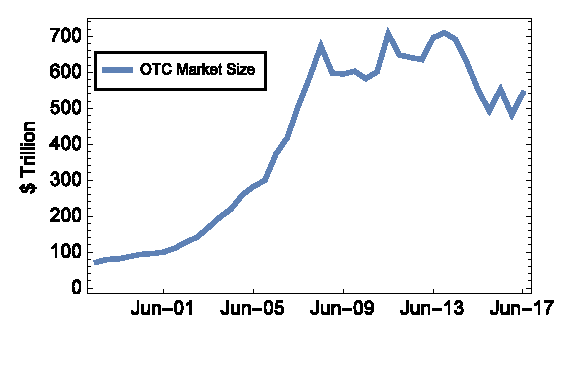
\includegraphics[width=.5\linewidth,trim={2pt 17pt 0 0},clip]{OTC.eps}
      \caption{Size of OTC derivatives market since May 1996.}\label{fig:OTC}
    \end{figure}

\section{Options}
\label{section:options}
Of all kinds of derivatives, in this master thesis we will focus particularly on the most traded one: options~\cite{Hull}.
As the name implies, an option contract grants its buyer the option to buy or sell its underlying asset within a given time frame, known as the expiration date.

\subsection{Call and Put Options}
\label{subsection:calls and puts}
The two main types of options are calls and puts. They grant their buyer the right to buy and sell the underlying asset, respectively, for a fixed price, known as the strike price, in the future.
It's important to emphasize the fact that an option grants its buyer the right to do something. If this action would lead to losses, a buyer can simply decide to let the expiration date pass, thus avoiding further losses. This is indeed the most attractive characteristic of options.

\subsection{European and American Options}
\label{subsection:european and american options}
Options are also categorized by the period at which the buyer is allowed to exercise his right. The two most traded types are European and American options.
With an European option, an investor is only able to exercise the contract at the expiration date. The value of the underlying asset up to that point in time is irrelevant.
As for American options, the buyer can exercise the contract at any moment up to the expiration date.
In this case, the investor is faced with an optimal-stopping problem: when is the best time to exercise the option?
For this very reason, it should be clear that American options are significantly more difficult to study than their European counterparts.

\subsection{Why Options are Important}
\label{subsection:why options are important}
Options are very useful tools to all investors. 
To hedgers (i.e. investors that want to limit their exposure to risk), options provide safety by fixing the future price of their underlying asset (e.g. if hedgers want to protect themselves against a potential price crash affecting one of their assets, they can buy put options on them. Now, even if the value their asset decreases significantly, their losses are contained because they can always exercise the options and sell the asset at the option's higher strike price).

To speculators (i.e. investors that want to take advantage of the uncertainty of future markets by speculating on their outcome), options grant access to much higher profits (e.g. if speculators strongly believe that the value of a given asset will greatly increase in the future, they can buy call options on that asset. If their prediction proves right, they can buy that asset for the option's lower strike price).

Due to all their advantages, and unlike some other types of derivatives, options have a cost. Finding the ideal price for an option is a fundamental concern to investors, since knowing its true value can give them a chance to take advantage of an under or overpriced option.
Finding this price can be very difficult for some options, however. Though a lot of research has been done towards this goal, a great deal more is still required.


\section{Topic Overview}
\label{section:overview}

Provide an overview of the topic to be studied...


\section{Objectives}
\label{section:objectives}

Explicitly state the objectives set to be achieved with this thesis...


\section{Thesis Outline}
\label{section:outline}

Briefly explain the contents of the different chapters...

 % file "Thesis_Introduction.tex"
\cleardoublepage

%%%%%%%%%%%%%%%%%%%%%%%%%%%%%%%%%%%%%%%%%%%%%%%%%%%%%%%%%%%%%%%%%%%%%%%%
%                                                                      %
%     File: Thesis_Background.tex                                      %
%     Tex Master: Thesis.tex                                           %
%                                                                      %
%     Author: Andre C. Marta                                           %
%     Last modified :  2 Jul 2015                                      %
%                                                                      %
%%%%%%%%%%%%%%%%%%%%%%%%%%%%%%%%%%%%%%%%%%%%%%%%%%%%%%%%%%%%%%%%%%%%%%%%

\chapter{Background}
\label{chapter:background}

Insert your chapter material here...


%%%%%%%%%%%%%%%%%%%%%%%%%%%%%%%%%%%%%%%%%%%%%%%%%%%%%%%%%%%%%%%%%%%%%%%%
\section{Theoretical Overview}
\label{section:overview}

Some overview of the underlying theory about the topic...


%%%%%%%%%%%%%%%%%%%%%%%%%%%%%%%%%%%%%%%%%%%%%%%%%%%%%%%%%%%%%%%%%%%%%%%%
\section{Theoretical Model 1}
\label{section:theory1}

The research should be supported with a comprehensive list of references.
These should appear whenever necessary, in the limit, from the first to the last chapter.

A reference can be cited in any of the following ways:
%
\begin{itemize}
  \item Citation mode \#1 - \quad \cite{jameson:adjointns}
  \item Citation mode \#2 - \quad \citet{jameson:adjointns}
  \item Citation mode \#3 - \quad \citep{jameson:adjointns}
  \item Citation mode \#4 - \quad \citet*{jameson:adjointns}
  \item Citation mode \#5 - \quad \citep*{jameson:adjointns}
  \item Citation mode \#6 - \quad \citealt{jameson:adjointns}
  \item Citation mode \#7 - \quad \citealp{jameson:adjointns}
  \item Citation mode \#8 - \quad \citeauthor{jameson:adjointns}
  \item Citation mode \#9 - \quad \citeyear{jameson:adjointns}
  \item Citation mode \#10 - \quad \citeyearpar{jameson:adjointns}
\end{itemize}
%
Several citations can be made simultaneously as \citep{nocedal:opt,marta:ijcfd}. \\

This is often the default bibliography style adopted (numbers following the citation order), according to the options:\\
{\tt \textbackslash usepackage\{natbib\}} in file {\tt Thesis\_Preamble.tex},\\
{\tt \textbackslash bibliographystyle\{abbrvnat\}} in file {\tt Thesis.tex}.\\

Notice however that this style can be changed from numerical citation order to authors' last name with the options: \\
{\tt \textbackslash usepackage[numbers]\{natbib\}} in file {\tt Thesis\_Preamble.tex},\\
{\tt \textbackslash bibliographystyle\{abbrvunsrtnat\}} in file {\tt Thesis.tex}. \\

Multiple citations are compressed when using the {\tt sort\&compress} option when loading the {\tt natbib} package as {\tt \textbackslash usepackage[numbers,sort\&compress]\{natbib\}} in file {\tt Thesis\_Preamble.tex}, resulting in citations like \citep{marta:ijcfd1,marta:ijcfd2,marta:ijcfd3,marta:ijcfd4}.


%%%%%%%%%%%%%%%%%%%%%%%%%%%%%%%%%%%%%%%%%%%%%%%%%%%%%%%%%%%%%%%%%%%%%%%%
\section{Theoretical Model 2}
\label{section:theory2}

Other models...

 % file "Thesis_Background.tex"
\cleardoublepage

\chapter{Volatility}
\label{chapter:volatility}
As mentioned, volatility is a measure of the uncertainty of future stock price movements. In other words, a higher volatility will lead to greater future fluctuations in the stock price, whereas a stock with lower volatility is more stable. This phenomenon is exemplified in \autoref{fig:VarVol}, where we can see the greater fluctuations of the high-volatility process (red) compared to the much smaller variations of the low-volatility process (orange), using the same driving Brownian motion.
\begin{figure}[!htb]
    \centering
      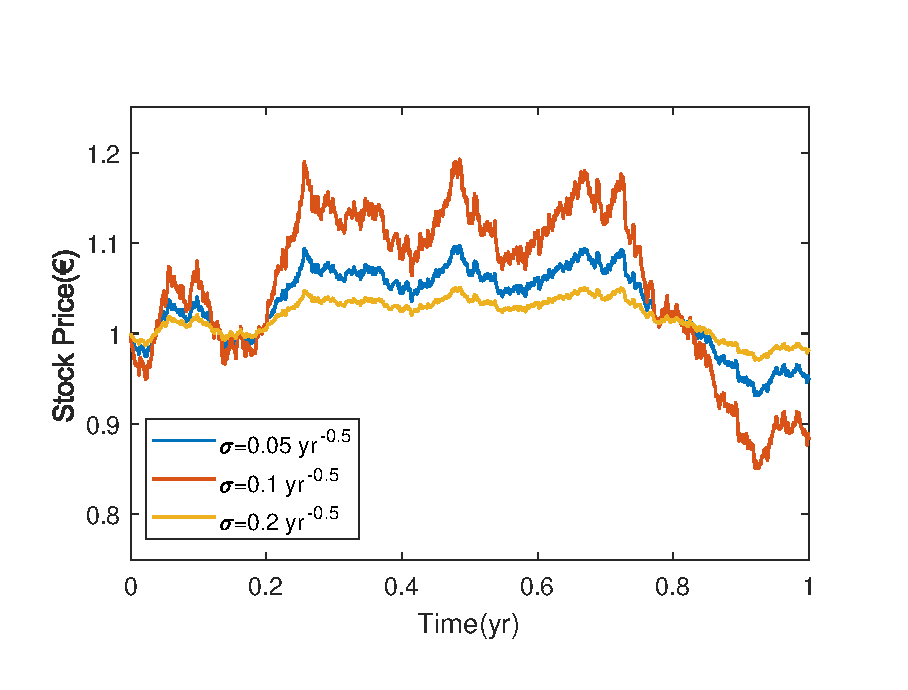
\includegraphics[width=.65\columnwidth]{VarVol.eps}
      \caption[Example of three identical GBM processes with different volatilities]{Example of three identical GBM processes with maturity $T=\SI{1}{\year}$, interest rate $r=\SI{0.01}{\per\year}$ and initial stock price $S_0=\SI{1}{\EUR}$. The volatilities are $\sigma=\SI{0.05}{\year\tothe{-1/2}}$, $\sigma=\SI{0.1}{\year\tothe{-1/2}}$ and $\sigma=\SI{0.2}{\year\tothe{-1/2}}$ for the orange, blue and red plot lines represented, respectively. To emphasize this effect, the underlying Brownian Motion $\{W(t),\ t>0\}$ used to generate all three paths was the same.}\label{fig:VarVol}
    \end{figure}

Of all the parameters in the BS formula (eq.\eqref{BS2}), volatility is the only one we can't easily measure from market data.
Furthermore, unlike the interest rate, volatility has a great impact on the behavior of stock prices and, consequently, on the price of options~\citep{Wilmott3}.
These two factors make volatility one of the most important subjects in all of mathematical finance and thus the focus of much research.

Usually, volatility can be estimated empirically from the standard deviation of the historical rate of log-returns~\citep{Hull}.
We begin by measuring the stock price at fixed time intervals (e.g. daily, monthly), such that $S_i$ corresponds to the stock price at the end of the $i$th interval. We define the log-return rate, $u_i$, as
\begin{equation}
u_i=\log\left(\frac{S_i}{S_{i-1}}\right).
\end{equation}
We can then calculate the standard deviation, $s$, of this rate as
\begin{equation}
s=\sqrt{\frac{1}{n-1}\sum_{i=1}^n(u_i-\overline{u})^2},
\end{equation}
\noindent assuming we have $n+1$ observations and denoting $\overline{u}$ as the average value of the log-return rates.
The volatility (measured yearly) can be \emph{estimated} with
\begin{equation}
\hat{\sigma}=\frac{s}{\sqrt{\tau}},
\end{equation}
\noindent where $\tau$ defines the time interval length measured in years. As an example, if we only have monthly data for the $S_i$ prices, the time interval would obviously be one month, which, measured in years is equal to $1/12$, which corresponds to $\tau$.
The volatility can also be measured in other time periods: we can define a monthly or a daily volatility, instead of a yearly volatility as we defined before, but these are less common and will therefore not be used.

We are now able to estimate the volatility of any given asset at the present moment. With this result, we could assume that the volatilities remain constant over time and use today's volatility to price options with maturities in the future. The clear problem with this approach is that, when observing market data, we can see that volatilities change over time, so that even if we had the exact value of this parameter in the present, it can, and will, change in the future. If we try to price options assuming a constant volatility, our options will become mispriced, causing potential losses.
Our goal is therefore to model the volatility of any given stock price, and, with this model, predict its future behavior, using this knowledge to better price options.
We begin by introducing the concept of implied volatility, crucial to fully grasping the concepts used later. Afterwards, we will introduce four models to replicate market volatility: one with local volatility (Dupire's formula) and three with stochastic volatility (Heston and Static/Dynamic SABR).

We should note that other very common models exist. The GARCH model (Generalized Autoregressive Conditional Heteroskedasticity) along with all its many variations (EGARCH, NGARCH, ...) is particularly popular among econometricians. However, this model is mostly used to forecast volatility, and performs poorly when used to price derivatives~\citep{chourdakis}. Because pricing is our objective, GARCH will not be covered in this work. We will also study the constant volatility model, as used by Black \textit{et al.}, as a benchmark for the quality of our models.



\section{Implied Volatility}
\label{section:impliedvolatility}
\emph{Implied volatility} can be described as the value of stock price volatility that, when input into the BS pricer in eq.\eqref{callputBS}, outputs a value equal to the market price of a given option.
In other words, it would be the stock price volatility that the seller/buyer of the option used when pricing it (assuming the BS model was used).

Because eq.\eqref{callputBS} is not invertible w.r.t. $\sigma$, we need to use some numerical procedure (e.g. Newton's method) to find the value of implied volatility that matches the market and model prices, i.e. we must find, numerically, the solution to the equation
\begin{equation}\label{impvolform}
C(\sigma_{imp})=C_{\mathrm{mkt}},
\end{equation}
\noindent where $C(\sigma_{imp})$ corresponds to the result of eq.\eqref{callputBS} using $\sigma_{imp}$ as (implied) volatility and $C_{\mathrm{mkt}}$ to the price of the option observed in the market.



Solving eq.\eqref{impvolform} to find the implied volatility of different option market prices, we find the relationship depicted in \autoref{fig:ImpVolPrice}, for three different strike prices.


\begin{figure}[H]
    \centering
      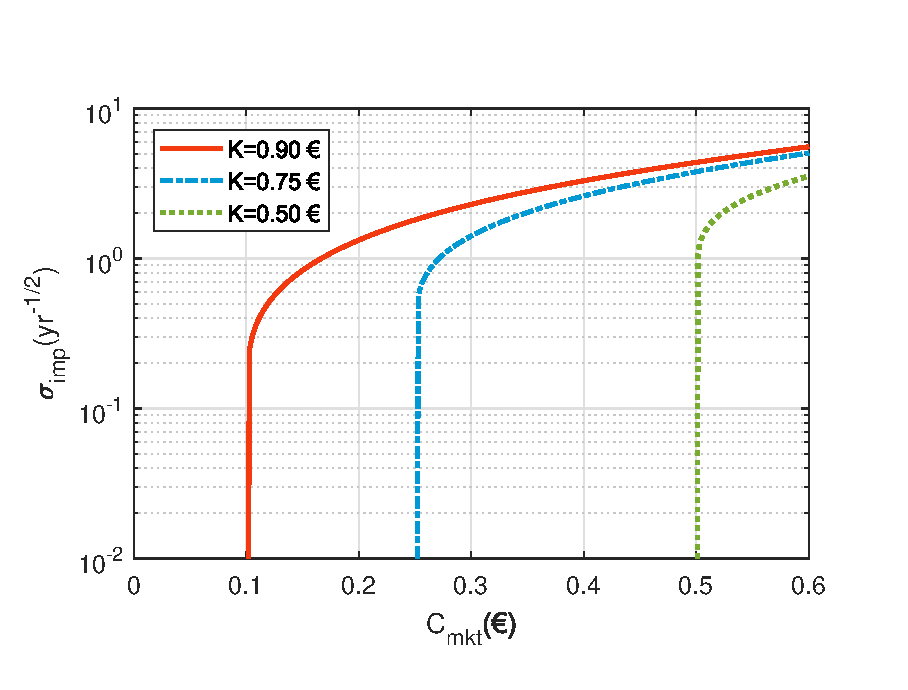
\includegraphics[width=.65\columnwidth]{ImpVolC.eps}
      \caption[Relationship between the implied volatility and the market price of a call option.]{Relationship between the implied volatility and the market price of a call option. The parameters used were $T=21$ days, interest rate $r=\SI{0.01}{\per\year}$ and initial stock price $S_0=\SI{1}{\EUR}$. The strike prices are $K=\SI{0.9}{\EUR}$, $K=\SI{0.75}{\EUR}$ and $K=\SI{0.5}{\EUR}$ for the red full line, the blue dot-dashed line and the green dot-dashed line, respectively.}\label{fig:ImpVolPrice}
    \end{figure}

We can see that the implied volatility goes to zero extremely fast when we approach the lower bound of the call option's price, $S_0-Ke^{-rT}$ (from eq.\eqref{bound}) - the lower bounds for the option prices with strikes $K=\SI{0.9}{\EUR}$, $K=\SI{0.75}{\EUR}$ and $K=\SI{0.5}{\EUR}$ are, respectively, $C=\SI{0.1007}{\EUR}$, $C=\SI{0.2506}{\EUR}$ and $C=\SI{0.5004}{\EUR}$). We can thus conclude that the implied volatility is extremely sensitive to the option's market price when this price approaches its lower bound. We can also observe that this property is more pronounced for lower strikes. This observation will become very important in later sections.

From \autoref{fig:ImpVolPrice} we can also observe that the relation between implied volatility and market option price is a monotonous increasing function.
This means that we can obtain the implied volatility of an option from its price and vice versa (i.e. the relationship is bijective). This duality is so fundamental that investors often disclose options by providing their implied volatility instead of their price~\citep{Wilmott}, as is indeed the case for the data we will use later to calibrate the models.
To understand why option price is an increasing monotonous function w.r.t. the volatility we note that volatility is very desirable to investors when dealing with options. A high volatility means that there is an increased probability that the stock price will increase or decrease very significantly. In the case of a call option, if the stock price increases considerably, the investor earns a large amount of money. If the price decreases considerably, the investor may let the option expire. Thus we see that a higher volatility provides a greater change of potentially very high profits with a limited potential downfall. We thus conclude that a higher volatility increases the value of an option.



One important property of implied volatility is that, in the real-world, it depends on the strike price and the maturity. This should not occur in the "Black-Scholes world". Because the volatility is a property of the stock, if investors really used the the BS model to price their options, two options with the same underlying stock should have the same implied volatility, regardless of their strike prices or maturities (i.e. the same stock can't have two different volatilities at the same time).
However, when observing real market data, this is in fact what is observed.

The implied volatilities' dependence on the strike price can take one of two forms, known as \emph{smile} and \emph{skew}.
An implied volatility smile presents higher volatilities for options with strikes farther from the current stock price (i.e. the shape of a smile). A skew, on the other hand, only presents higher volatilities in one of these directions (i.e. only for strikes either greater or smaller than the current stock price). Both phenomena are represented in \autoref{fig:smileskew}.
\begin{figure}[!htb]
  \begin{subfigmatrix}{2}
    \subfigure[Smile]{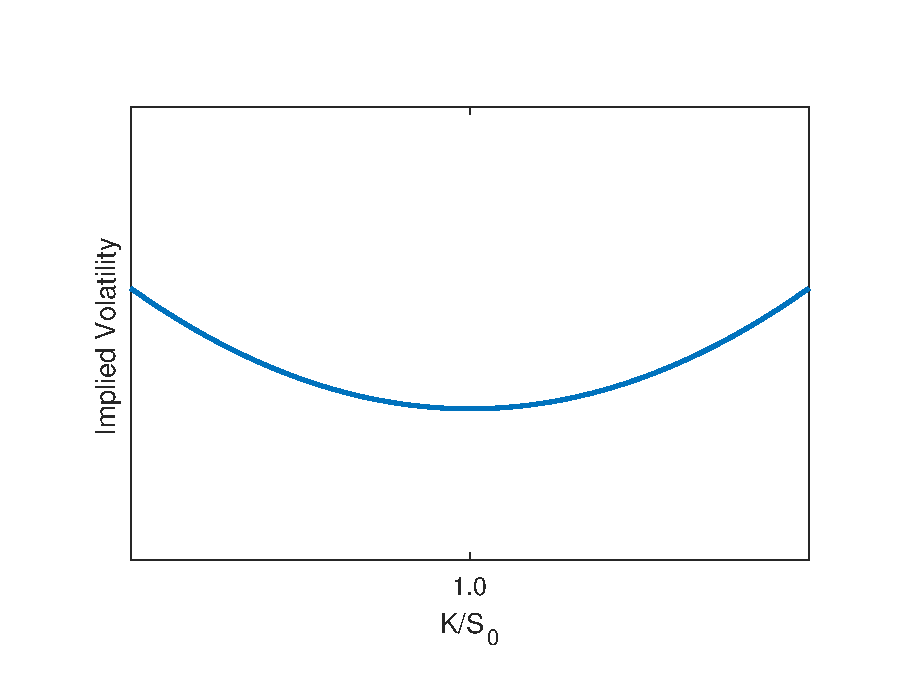
\includegraphics[width=0.49\linewidth]{Smile.eps}}
    \subfigure[Skew]{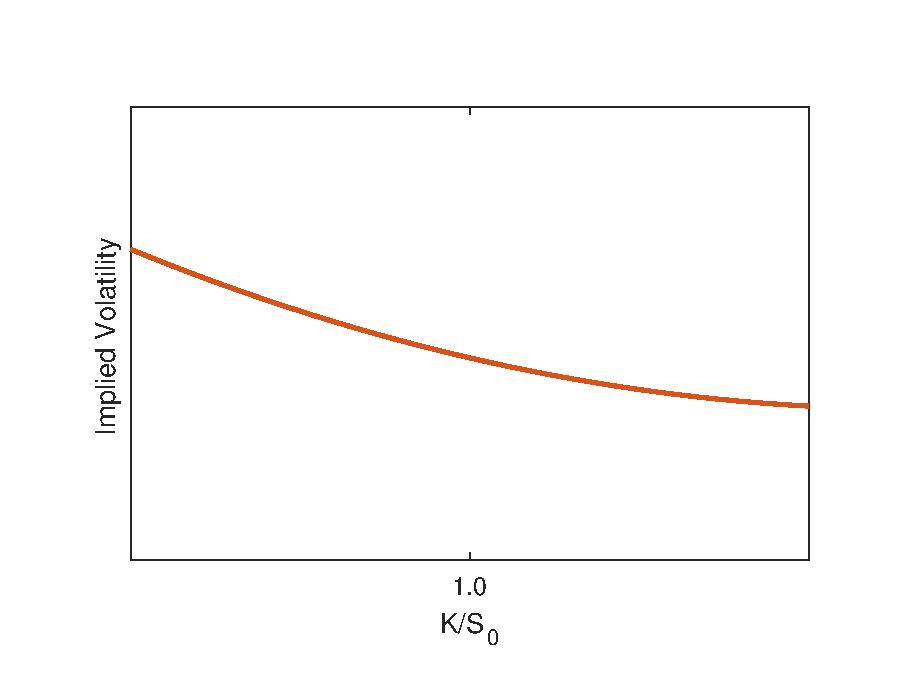
\includegraphics[width=0.49\linewidth]{Skew.eps}}
  \end{subfigmatrix}
  \caption[Representation of the implied volatility smile and skew functions.]{Representation of the implied volatility smile (left) and skew (right) functions.}
  \label{fig:smileskew}
\end{figure}


Because of their higher implied volatility, we can conclude that, if we observe a smile in the data, options with strikes different from the current stock price are \emph{overpriced}.
The reason behind this odd market behavior is related to the simple demand-supply rule~\citep{Wilmott3}. On the one hand, some investors are risk-averse and want to hedge their losses in case of a big market movement (as explained in \autoref{subsection:why options are important}). They don't mind paying a higher price for an option if this means they would be relatively safe from potentially devastating price changes. For this reason, the demand of call options with lower strikes increases, driving their prices and, consequently, their implied volatility up. On the other hand, other investors are risk-seekers and want to take advantage of possible sudden price movements, buying the stocks after the possible price increase for the lower strike prices. They don't mind paying higher prices for the chance of earning high profits and this drives the prices of high strike call options and, consequently, their implied volatility up. This fear-greed duality gives rise to the observed volatility smile. 
In the case of the volatility skew, only one of the two phenomena described occurs.


The presence of a smile in the data instead of a skew, and vice-versa, is determined by the type of product serving as underlying asset - Forex market options usually exhibit volatility smiles whereas index and commodities options usually show a volatility skew or a skewed smile~\citep{Wilmott3}.

The dependence of the implied volatility on the maturity date is more complex, but in general it decreases with the maturity.

It can also be shown that the implied volatility is the same for calls and puts~\citep{Hull}, though the causes of the volatility smile/skew for put options are the opposite of the ones described before for calls.






\section{Local Volatility}
\label{section:localvolatility}
In their original work, Black \textit{et al.} assumed that volatility is constant throughout the whole option duration. From market data, it can be clearly seen that this is not the case~\citep{DJIA}. There may be times when new information reaches the market  (e.g. the results of an election) and trading increases, driving volatility up. It is equally true that shortly before this information is known, trading may stall due to expectancy, and volatilities go down. 

The constant volatility BS model is therefore clearly incapable of completely grasping real-world trading. We should use a model where volatility is dynamic, measuring the uncertainty on the stock price movement at any point in time.
However, as we saw in \autoref{section:impliedvolatility}, the market's view of volatility also depends on the stock price itself.
The volatility should therefore be a function of both time and stock price: $\sigma(S(t),t)$. We call this model \emph{local volatility} and the geometric Brownian motion from eq.\eqref{GBM} is transformed into the new diffusion process
\begin{equation}\label{GBM2}
dS(t)=rS(t)dt+\sigma(S(t),t)S(t)dW(t),
\end{equation}
\noindent where $\sigma(S(t),t)$ is a function of $S(t)$ and $t$, with certain properties, which we omit as they are only used to ensure the strong solution of this SDE (i.e. $\sigma(S(t),t)$ is "well behaved").


This local volatility model implies that we have a nonlinear \emph{deterministic} volatility surface, $\sigma(S(t),t)$, which can be thought of as the market's expectation of future volatility at time $t$ if the stock price is $S(t)$ at that time.



Because we can't directly measure the local volatility of a stock from market data, we need some models to estimate it. One of the most used of these is known as Dupire's formula, which we explain in the following subsection.


\subsection{Dupire's model}
\label{subsection:Dupire}
One of the most famous results in the modelling of the local volatility function was obtained by Dupire~\citep{Dupire}. In his article, this author derives a theoretical formula for $\sigma(S(t),t)$, given by
\begin{equation}\label{dupire}
\sigma(S(t),t)=\sqrt{\frac{\displaystyle\pdv{C}{T}+rS\pdv{C}{K}}{\displaystyle\frac{1}{2}S^2\pdv{^2C}{K^2}}},
\end{equation}
\noindent where $C=C(K,T)$ is the price of an European call option with strike price $K$ and maturity $T$. All the derivatives are evaluated at $K=S(t)$ and $T=t$.



\begin{proof}

We begin by assuming that the stock price $S(t)$ follows a dynamic transition probability density function $p(S(t),t,S'(t'),t')$. In other words, by integrating this density function we would obtain the probability of the stock price reaching a price $S'$ at a time $t'$ having started at price $S$ at time $t$.

The present value of a call option, $C(K,T)$, can be deduced as its expected future payoff, discounted backwards in time, which results in
\begin{equation}
\begin{split}\label{deriv0}
C(K,T)=e^{-r(T-t)}\mathbb{E}\left[\max\left(S'-K,0\right)\right]&=e^{-r(T-t)}\int_0^\infty\max\left(S'-K,0\right)p(S,t,S',T)dS'\\
&=e^{-r(T-t)}\int_K^\infty(S'-K)p(S,t,S',T)dS',
\end{split}
\end{equation}
\noindent where $S'$ denotes the stock price at maturity.

Taking the first derivative of this result with respect to the strike price $K$, we obtain
\begin{equation}\label{dcdk}
\pdv{C}{K}=-e^{-r(T-t)}\int_K^\infty p(S,t,S',T)dS'.
\end{equation}
The second derivative results in
\begin{equation}\label{d2cdk2}
\pdv{^2C}{K^2}=e^{-r(T-t)}p(S,t,K,T),
\end{equation}
\noindent assuming $p(S,t,\infty,T)=0$.

We now make a brief detour to derive the Fokker-Planck equation (following the procedure shown in ~\citep{Wilmott}), which we require for the next steps. This equation is widely used in stochastic calculus, and is applicable to stochastic processes in general.
To make its proof simpler, we make a simplification assuming that the stochastic process is a stock price following a trinomial model: at each time step, the stock price can only increase or decrease by an amount $dS$, with probabilities $\phi^+$ and $\phi^-$, respectively, or remain the same, with probability $(1-\phi^+-\phi^-)$. The resulting equation still works, however, for any general stochastic process.


Assuming the trinomial model, the expected value of the change is given by
\begin{equation}
\phi^+dS+(1-\phi^+-\phi^-).0+\phi^-(-dS)=(\phi^+-\phi^-)dS,
\end{equation}
\noindent and its variance is approximately given by
\begin{equation}
(dS)^2(\phi^++\phi^--(\phi^+-\phi^-)^2)\approx (\phi^++\phi^-)(dS)^2
\end{equation}
\noindent where we take only the first order terms. The expected value of the change of a GBM can be thought of as its drift term (i.e. $rSdt$), and the variance is its stochastic term squared (i.e. $(\sigma SdW)^2=\sigma^2S^2dt$), so that we have
\begin{equation}
\begin{split}
rSdt&=(\phi^+-\phi^-)dS;\\
\sigma^2S^2dt&=(\phi^++\phi^-)(dS)^2,
\end{split}
\end{equation}
\noindent from which we can derive the probabilities $\phi^+$ and $\phi^-$ as
\begin{equation}
\begin{split}
\phi^+&=\frac{1}{2}\frac{dt}{dS^2}(rSdS+\sigma^2S^2);\\
\phi^-&=\frac{1}{2}\frac{dt}{dS^2}(-rSdS+\sigma^2S^2).
\end{split}
\end{equation}

We can now move backwards and derive the probability of reaching the price $S'$ at time $t'$ having started at the previous time $t'-dt$ with some (unknown) price $S$, which could be either $S'+dS$, $S'-dS$ or $S'$ (assuming a trinomial movement). This probability is indeed the probability density, $ p(S,t,S',T) $ and can be derived as
\begin{equation}
p(S,t,S',T)=\phi^-p(S'+dS,t-dt,S',T)+(1-\phi^+-\phi^-)(S',t-dt,S',T)+\phi^+p(S'-dS,t-dt,S',T).
\end{equation}
\noindent If we expand each term on its Taylor series around point $(S',t')$, we get
\begin{equation}
\begin{split}
p(S,t,S',T)=&\ \phi^-\left(p(S',t,S',T)+dS\frac{dp}{dS'}+\frac{1}{2}(dS)^2\frac{d^2p}{dS^2}-dt\frac{dp}{dt'}\right)\\
&+(1-\phi^+-\phi^-)\left(p(S',t,S',T)-dt\frac{dp}{dt'}\right)\\
&+\phi^+\left(p(S',t,S',T)-dS\frac{dp}{dS'}+\frac{1}{2}(dS)^2\frac{d^2p}{dS^2}-dt\frac{dp}{dt'}\right)\\
=&\frac{1}{2}\frac{dt}{dS'^2}\sigma^2S'^2(dS)^2\frac{d^2p}{dS'^2}-\frac{dt}{dS'^2}rS'(dS)^2\frac{dp}{dS'},
\end{split}
\end{equation}
\noindent from which we can derive the famous Fokker-Planck equation (with rather sloppy notation) as
\begin{equation}\label{FokkerPlanck}
\pdv{p}{T}=\frac{1}{2}\pdv{^2(\sigma^2S'^2p)}{S'^2}-\pdv{(rS'p)}{S'}.
\end{equation}
\noindent where we have used $t'=T$.


From eq.\eqref{deriv0} we can easily obtain the first derivative w.r.t. time
\begin{equation}
\pdv{C}{T}=-rC+e^{-r(T-t)}\int_K^\infty(S'-K)\pdv{p}{T}dS',
\end{equation}
\noindent where, for simplicity, we drop the terms of the transition probability density, $p$.

Using the Fokker-Planck formula in eq.\eqref{FokkerPlanck}, we can transform this relation into
\begin{equation}
\pdv{C}{T}=-rC+e^{-r(T-t)}\int_K^\infty(S'-K)\left(\frac{1}{2}\pdv{^2(\sigma^2S'^2p)}{S'^2}-r\pdv{(S'p)}{S'}\right)dS'.
\end{equation}

We now split the terms in the integral to evaluate them independently. We integrate the second term by parts as
\begin{equation}
\begin{split}
\int_K^\infty(S'-K)\left(-r\pdv{(S'p)}{S'}\right)dS'&=-r(S'-K)(S'p)\big|_{S'=K}^\infty+r\int_K^\infty S'p dS'\\
&=r\int_K^\infty (S'-K)p dS'+rK\int_K^\infty p dS'\\
&=e^{r(T-t)}rC-rK\pdv{C}{K}
\end{split}
\end{equation}
\noindent where in the first step we assumed that $p$ and its first derivative w.r.t. $S$ go sufficiently fast to zero when $S$ goes to infinity and where in last step we used eqs.\eqref{deriv0} and\eqref{dcdk}.

Turning now to the first term of the integral, we integrate twice by parts as
\begin{equation}
\begin{split}
\int_K^\infty(S'-K)\left(\frac{1}{2}\pdv{^2(\sigma^2S'^2p)}{S'^2}\right)dS'&=\frac{1}{2}(S'-K)\pdv{(\sigma^2S'^2p)}{S'}\bigg|_{S'=K}^\infty-\frac{1}{2}\int_K^\infty\left(\pdv{(\sigma^2S'^2p)}{S'}\right)dS'\\
&=-\frac{1}{2}\sigma^2S'^2p\big|_{S'=K}^\infty=\frac{1}{2}\sigma^2(K,T)K^2p(S,t,K,T)\\
&=\frac{1}{2}e^{r(T-t)}\sigma^2(K,T)K^2\pdv{^2C}{K^2},
\end{split}
\end{equation}
\noindent where in the last step we used eq.\eqref{d2cdk2} and again assumed that $p$ goes to zero sufficiently fast.

Collecting all the terms, we obtain
\begin{equation}
\pdv{C}{T}=\frac{1}{2}\sigma^2(K,T)K^2\pdv{^2C}{K^2}-rK\pdv{C}{K}.
\end{equation}
\noindent from which, by rearranging all the terms and applying the variable change $\sigma(K,T)\implies \sigma(S,t)$, we get
\begin{equation}
\sigma(S(t),t)=\sqrt{\frac{\displaystyle\pdv{C}{T}+rS\pdv{C}{K}}{\displaystyle\frac{1}{2}S^2\pdv{^2C}{K^2}}}.
\end{equation}
\noindent assuming all the derivatives are evaluated at $K=S(t)$ and $T=t$.

\end{proof}

As can be seen, we need to differentiate the option prices with respect to their strikes and maturities. To achieve this, we need first to gather, from the market, a large number of prices for options with different maturities and strikes. We then implement some interpolation on these values to obtain an option price surface (with $K$ and $T$ as variables). Finally, we calculate the gradients of this interpolated surface and input them into eq.\eqref{dupire} to obtain the local volatility surface.
We can then sample from this surface to obtain the local volatility for any stock price $S(t)$ at any time $t$.


A major problem can be pointed out in eq.\eqref{dupire}. For options far in or far out of the money (i.e. with strikes much greater or much smaller that $S_0$), it can be shown that the option price depends almost linearly on the strike. This means that the second derivative of the price w.r.t. the strike is extremely small in these regions. Because this value is in the denominator of eq.\eqref{dupire}, the local volatility will explode in such cases, which is unrealistic.


One possible solution to this problem is to relate our local volatility with the implied volatility surface instead of the option price's~\citep{Wilmott}.
The relation obtained is
\begin{equation}\label{dupire2}
\boxed{\sigma(S(t),t)=\sqrt{\frac{\displaystyle\sigma_{imp}^2+2t\sigma_{imp}\pdv{\sigma_{imp}}{T}+2r(S(t))t\sigma_{imp}\pdv{\sigma_{imp}}{K}}{\displaystyle\left(1+(S(t))d_1\sqrt{t}\pdv{\sigma_{imp}}{K}\right)^2+(S(t))^2t\sigma_{imp}\left(\pdv{^2\sigma_{imp}}{K^2}-d_1\left(\pdv{\sigma_{imp}}{K}\right)^2\sqrt{t}\right)}},}
\end{equation}
\noindent where $d_1$ is given by
\begin{equation}
d_1=\frac{\log(S_0/S(t))+\left(r+\frac{1}{2}\sigma_{imp}^2\right)t}{\sigma_{imp}\sqrt{t}},
\end{equation}
\noindent with $S_0$ being the stock price at $t=0$. We define $\sigma_{imp}=\sigma_{imp}(K,T)$ as the implied volatilities of options with maturity $T$, and strike $K$. Furthermore, $\sigma_{imp}$ and all its derivatives are evaluated at $K=S(t)$ and $T=t$. This formula can be obtained from eq.\eqref{dupire} by applying the transformation from call prices to implied volatilities.


We now need to generate the implied volatility surface in order to obtain the gradients needed in eq.\eqref{dupire2} to generate the local volatility. Again, this surface can be obtained by interpolating between market data for several implied volatilities. The problem with this approach is that we only have access to market data for a very limited set of implied volatilities. This problem is therefore very much ill-posed (i.e. a small change in the input generates a very different output) and the resulting local volatility surface might look unrealistic~\citep{Wilmott}. Furthermore, this procedure is heavily dependent on the interpolation/extrapolation method chosen, which is problematic.

As an advantage, we note that because we are directly using the market data, the implied volatility surface is nonparametric and therefore no fitting procedure is required. To ease the problem of ill-posedness, we could heuristically choose some functions to model this surface, fitting their parameters to better replicate the market data, and finally replacing these functions in eq.\eqref{dupire2}, as done by Dewynne~\citep{dewynne}. However, this solution depends heavily on the functions chosen and will not be considered.



Three other problems can be identified in Dupire's local volatility model.
First, it can be shown that the local volatility surface changes with time~\citep{Wilmott}. This means that the whole interpolation procedure must be done regularly in order for the model to work properly.
Secondly, some authors have pointed out that the volatility smile obtained from Dupire's local-volatility model doesn't follow real market dynamics~\citep{Hagan}: it can be shown that when the price of the stock either increases or decreases, the volatility smile predicted by Dupire's model shifts in the opposite direction. The minimum of the volatility smile would therefore be offset and no longer correspond to the local stock price (i.e. the spot price). The volatility smile dynamics obtained from the local-volatility model would thus be actually worse than if we assumed a constant volatility.
Finally, the gradients used in eq.\eqref{dupire2} have to be generated numerically. This numerical differentiation is very unstable, especially when done on our rough interpolated surface, which might lead to errors in the local volatility obtained.

Despite its problems, Dupire's formula is still very much used by practitioners and performs surprisingly well, as we will see in \autoref{chapter:results}.



\section{Stochastic Volatility}
\label{section:stochastic volatility}
As stated before, the volatility is not constant, is not observable and is very unpredictable, despite our attempts to model it. This seems to indicate that volatility is itself also a stochastic process. Some research has been done into this hypothesis, and many models have been developed to replicate real-world volatilities with this assumption.

We assume that the stock price follows the diffusion process
\begin{equation}\label{stochvol}
dS(t)=rS(t)dt+\sigma(S(t),t)S(t)dW_1(t),
\end{equation}
\noindent and we further hypothesize that the volatility follows
\begin{equation}
d\sigma(S(t),t)=p(S(t),\sigma(S(t),t),t)dt+q(S(t),\sigma(S(t),t),t)dW_2(t),
\end{equation}
\noindent where $p(S(t),\sigma(S(t),t),t)$ and $q(S(t),\sigma(S(t),t),t)$ are functions of the stock price $S(t)$, time $t$ and of the volatility $\sigma(S(t),t)$ itself. We also assume that $W_1$ and $W_2$ are two Brownian motion processes with a correlation $\rho(t)$, i.e.
\begin{equation}
dW_1(t)dW_2(t)=\rho(t) dt, \ \ \ \forall t>0,
\end{equation}
\noindent which is usually assumed constant, $\rho(t)=\rho$. This correlation coefficient can be explained by the relationship between prices and volatilities~\citep{chourdakis}. Historically, we can see that high volatility periods usually occur when the market is under stress due to low returns (i.e. stock prices decrease).
On the other hand, whenever the market stabilizes and returns increase, the volatility goes down.
These factors seem to indicate the existence of a negative correlation between stock prices and volatilities. Thus, to fully grasp market behavior, this correlation must be taken into account.



Choosing the appropriate functions $p(S(t),\sigma(S(t),t),t)$ and $q(S(t),\sigma(S(t),t),t)$ is very important since the whole evolution of the stock price depends on them. All stochastic volatility models present a different version of these functions, and each may be more adequate for some types of assets. Furthermore, these functions have some parameters that we have to calibrate in order to best fit our model to market data, as we will see later.


Many stochastic volatility models exist, such as Hull-White~\citep{hullwhite} and Stein-Stein~\citep{stein}. However, the \emph{Heston} model is by far the most popular of these~\citep{chourdakis}.
Another model, known as \emph{SABR}, is also widely used by practitioners, especially in the interest rate derivative markets (i.e. derivatives whose underlying asset is an interest rate). For these reasons, both these models will be studied in this work.


\subsection{Heston Model}
The \emph{Heston model} was developed in 1993 by Steven Heston~\citep{Heston} and it states that stock prices satisfy the relations
\begin{equation}\label{hestons}
\boxed{dS(t)=rS(t)dt+\sqrt{\nu(t)}S(t)dW_1(t),}
\end{equation}
\begin{equation}\label{hestonv}
\boxed{d\nu(t)=\kappa(\overline{\nu}-\nu(t))dt+\eta\sqrt{\nu(t)}dW_2(t),}
\end{equation}
\noindent with $\nu(t)$ corresponding to the stock price variance (i.e. the square of the volatility, $\nu(t)=(\sigma(t))^2$) and where $W_1(t)$ and $W_2(t)$ have a constant correlation $\rho$. We furthermore define $\nu_0$ as the initial variance (i.e. variance at time $t=0$). The original model used a drift parameter $\mu$ instead of the risk-free measure drift $r$ presented here, but a measure transformation, using Gisarnov's theorem, can be easily implemented~\citep{rouah}.

The parameters $\kappa$, $\overline{\nu}$ and $\eta$ are, respectively, the \emph{mean-reversion rate} (i.e. how fast the variance converges to its mean value), the \emph{long-term variance} (i.e. the mean value of variance) and the \emph{volatility of the variance} (i.e. how erratic is the variance process).



One of the reasons why the Heston model is so popular is the fact that there exists a closed-form solution for the prices of European options priced under this model. This closed form solution is given by
\begin{equation}\label{CH}
\begin{split}
C_{H}(K,T;\theta)&=e^{-rT}\mathbb{E}\left[\left(S(T)-K\right)\mathbbm{1}_{\left\{S(T)>K\right\}}\ \vert\ \theta\right]\\
&=e^{-rT}\left(\mathbb{E}\left[S(T)\mathbbm{1}_{\left\{S(T)>K\right\}}\ \vert\ \theta\right]-K\mathbb{E}\left[\mathbbm{1}_{\left\{S(T)>K\right\}}\ \vert\ \theta\right]\right)\\
&=S_0P_1(K,T;\theta)-e^{-rT}KP_0(K,T;\theta),
\end{split}
\end{equation}
\noindent where $C_{H}(K,T;\theta)$ corresponds to the theoretical European call option price, with strike $K$ and maturity $T$, under the Heston model, assuming a parameter set $\theta=\left\{\kappa,\overline{\nu},\eta,\nu_0,\rho\right\}$. The variables $P_1(K,T;\theta)$ and $P_2(K,T;\theta)$ are given by
\begin{equation}\label{P1}
P_1(K,T;\theta)=\frac{1}{2}+\frac{1}{\pi}\int_0^\infty\operatorname{Re}\left(\frac{e^{-iu\log K}}{iuS_0e^{rT}}\phi(u-i,T;\theta)\right)du,
\end{equation}
\begin{equation}\label{P2}
P_0(K,T;\theta)=\frac{1}{2}+\frac{1}{\pi}\int_0^\infty\operatorname{Re}\left(\frac{e^{-iu\log K}}{iu}\phi(u,T;\theta)\right)du,
\end{equation}
\noindent where $i$ is the imaginary unit and $\phi(u,t;\theta)$ is the characteristic function of the logarithm of the stock price process (the characteristic function of a random variable is the Fourier transform of the probability density function of that variable).


It is crucial to define the appropriate characteristic function $\phi(u,t;\theta)$ in order to evaluate the integrals in eqs.\eqref{P1} and\eqref{P2} and, with them, find the option price with eq.\eqref{CH}. In his original article, Heston proposed a solution to this very characteristic function~\citep{Heston}. However, some posterior authors demonstrated that, for large maturities, some discontinuities appeared for the proposed solution~\citep{Kahl}. One possible alternative, proposed by Schoutens~\citep{Schoutens}, avoids this shortcoming and is given by
\begin{equation}\label{charfuncschoutens}
\phi(u,t;\theta)=\exp\left\{iu\left(\log S_0+rt\right)+\frac{\kappa\overline{\nu}}{\eta^2}\left[\left(\xi-\alpha\right)t-2\log\left(\frac{1-ge^{-\alpha t}}{1-g}\right)\right]+\frac{\nu_0}{\eta^2}\left(\xi-\alpha\right)\frac{1-e^{-\alpha t}}{1-ge^{-\alpha t}}\right\},
\end{equation}
\noindent where we define
\begin{equation}\label{xi}
\xi=\kappa-\eta\rho iu,
\end{equation}
\begin{equation}\label{alpha}
\alpha=\sqrt{\xi^2+\eta^2(u^2+iu)},
\end{equation}
\begin{equation}
g=\frac{\xi-\alpha}{\xi+\alpha}.
\end{equation}


\begin{proof}
We will follow the derivation presented in Gatheral~\citep{gatheral} with slight changes of variables, for consistency.

We begin by defining the (call) option's value equation (from Itô's Lemma) as
\begin{equation}\label{hestonproof1}
\pdv{C}{t}+\frac{1}{2}\nu S^2\pdv[2]{C}{S}+\rho\eta\nu S\pdv{C}{\nu}{S}+\frac{1}{2}\eta^2\nu\pdv[2]{C}{\nu}+rS\pdv{C}{S}-rC+\kappa(\overline{\nu}-\nu)\pdv{C}{\nu}=0.
\end{equation}

We now define the forward price as $F(t)=S(t)e^{r(T-t)}$, and introduce the variables $\tau=T-t$ and $x(t)=\log\left(F(t)/K\right)$. We furthermore denote $C^*$ as the future value to expiration of the option price (i.e. $C^*=Ce^{rT}$). The relation in eq.\eqref{hestonproof1} reduces to
\begin{equation}\label{hestonproof2}
-\pdv{C^*}{\tau}+\frac{1}{2}\nu\pdv[2]{C^*}{x}+\rho\eta\nu\pdv{C^*}{x}{\nu}+\frac{1}{2}\eta^2\nu\pdv[2]{C^*}{\nu}-\frac{1}{2}\nu\pdv{C^*}{x}+\kappa(\overline{\nu}-\nu)\pdv{C^*}{\nu}=0,
\end{equation}
\noindent which has a solution of the form ~\citep{duffie}
\begin{equation}\label{hestonproof3}
C^*(x,\nu,\tau)=Ce^{rT}=\left(S_0P_1-e^{-rT}KP_0\right)e^{rT}=K\left[e^xP_1(x,\nu,\tau)-P_0(x,\nu,\tau)\right].
\end{equation}


Substituting the solution of eq.\eqref{hestonproof3} in eq.\eqref{hestonproof2} implies that $P_0$ and $P_1$ must satisfy
\begin{equation}\label{hestonproof4}
-\pdv{P_j}{\tau}+\frac{1}{2}\nu\pdv[2]{P_j}{x}-\left(\frac{1}{2}-j\right)\nu\pdv{P_j}{x}+\frac{1}{2}\eta^2\nu\pdv[2]{P_j}{\nu}+\rho\eta\nu\pdv{P_j}{x}{\nu}+\left(\kappa(\overline{\nu}-\nu)+j\nu\rho\eta\right)\pdv{P_j}{\nu}=0,
\end{equation}
\noindent for $j=0,1$ and subject to the terminal condition $P_j(x,\nu,\tau=0)=\mathbbm{1}_{\left\{x>0\right\}}$.


To solve this problem we use a Fourier transform technique. Defining $\tilde{P_j}$ as the Fourier transform of $P_j$,
\begin{equation}
\tilde{P_j}(u,\nu,\tau)=\int_{-\infty}^{\infty}e^{-iux}P_j(x,\nu,\tau)dx,
\end{equation}
\noindent and substituting this result in eq.\eqref{hestonproof4} produces
\begin{equation}\label{hestonproof5}
\nu\left\{\omega_j\tilde{P_j}-\beta_j\pdv{\tilde{P_j}}{\nu}+\frac{\eta^2}{2}\pdv[2]{\tilde{P_j}}{\nu}\right\}+\kappa\overline{\nu}\pdv{\tilde{P_j}}{\nu}-\pdv{\tilde{P_j}}{\tau}=0,
\end{equation}
\noindent with
\begin{equation}
\omega_j=-\frac{u^2}{2}-\frac{iu}{2}+iju,
\end{equation}
\begin{equation}
\beta_j=\kappa-\rho\eta iu-\rho\eta j.
\end{equation}


Heston proposed that $\tilde{P_j}$ is a function of the form
\begin{equation}
\tilde{P_j}(u,\nu,\tau)=\frac{1}{iu}\exp\left\{\zeta_j(u,\tau)\overline{\nu}+\psi_j(u,\tau)\nu\right\}.
\end{equation}

We can therefore derive
\begin{equation}
\pdv{\tilde{P_j}}{\tau}=\left\{\overline{\nu}\pdv{\zeta_j}{\tau}+\nu\pdv{\psi_j}{\tau}\right\}\tilde{P_j},
\end{equation}
\begin{equation}
\pdv{\tilde{P_j}}{\nu}=\psi_j\tilde{P_j},
\end{equation}
\begin{equation}
\pdv[2]{\tilde{P_j}}{\nu}=\psi_j^2\tilde{P_j}.
\end{equation}

Thus, eq.\eqref{hestonproof5} is only satisfied if
\begin{equation}
\pdv{\zeta_j}{\tau}=\kappa\psi_j,
\end{equation}
\begin{equation}
\pdv{\psi_j}{\tau}=\omega_j-\beta_j\psi_j+\frac{\eta^2}{2}\psi_j^2.
\end{equation}

Integrating these solutions with terminal conditions $\zeta_j(u,0)=\psi_j(u,0)=0$, yields
\begin{equation}
\zeta_j(u,\tau)=\frac{\kappa}{\eta^2}\left[\left(\beta_j-\gamma_j\right)\tau-2\log\left(\frac{1-g_je^{-\gamma_j \tau}}{1-g_j}\right)\right],
\end{equation}
\begin{equation}
\psi_j(u,\tau)=\frac{1}{\eta^2}\left(\beta_j-\gamma_j\right)\frac{1-e^{-\gamma_j \tau}}{1-g_je^{-\gamma_j \tau}},
\end{equation}
\noindent where we define
\begin{equation}
\gamma_j=\sqrt{\beta_j-2\omega_j\eta^2},
\end{equation}
\begin{equation}
g_j=\frac{\beta_j-\gamma_j}{\beta_j+\gamma_j}.
\end{equation}

We finally arrive at the solution for $P_j$ given by
\begin{equation}
P_j(x,\nu,\tau)=\frac{1}{2}+\frac{1}{\pi}\int_0^\infty\operatorname{Re}\left(\frac{\exp\left\{\zeta_j(u,\tau)\overline{\nu}+\psi_j(u,\tau)\nu+iux\right\}}{iu}\right)du.
\end{equation}

A change of variables is possible, as shown by Crisostomo~\citep{Crisostomo}, such that the two different characteristic functions for $P_1$ and $P_0$ can be transformed into a single one by defining
\begin{equation}
P_1=\frac{1}{2}+\frac{1}{\pi}\int_0^\infty\operatorname{Re}\left(\frac{e^{-iu\log K}}{iuS_0e^{rT}}\phi(u-i,T;\theta)\right)du,
\end{equation}
\begin{equation}
P_0=\frac{1}{2}+\frac{1}{\pi}\int_0^\infty\operatorname{Re}\left(\frac{e^{-iu\log K}}{iu}\phi(u,T;\theta)\right)du,
\end{equation}
\noindent with the characteristic function $\phi(u,T;\theta)$ given by
\begin{equation}
\phi(u,t;\theta)=\exp\left\{iu\left(\log S_0+rt\right)+\frac{\kappa\overline{\nu}}{\eta^2}\left[\left(\xi-\alpha\right)t-2\log\left(\frac{1-ge^{-\alpha t}}{1-g}\right)\right]+\frac{\nu_0}{\eta^2}\left(\xi-\alpha\right)\frac{1-e^{-\alpha t}}{1-ge^{-\alpha t}}\right\}.
\end{equation}

\end{proof}



The main problem with the characteristic function presented in eq.\eqref{charfuncschoutens} is the fact that it is highly nonlinear. Because we will apply some optimization procedure to minimize the difference between the model and the market option prices (i.e. calibration), the optimizer is very likely become stuck in some local minimum and not find the globally optimal solution.
This shortcoming led some authors to propose several modified versions of this function, such as Rollin \textit{et al.}~\citep{Rollin}. Most recently, Cui \textit{et al.}~\citep{Cui} presented a characteristic function that not only doesn't have the previously mentioned discontinuities but also solves the nonlinearity problem, given by
\begin{equation}
\phi(u,t;\theta)=\exp\left\{iu\left(\log S_0+rt\right)-\frac{t\kappa\overline{\nu}\rho iu}{\eta}-\nu_0A+\frac{2\kappa\overline{\nu}}{\eta^2}D\right\},
\end{equation}
\noindent with $A$ and $D$ given by
\begin{equation}
A=\frac{A_1}{A_2},
\end{equation}
\begin{equation}
D=\log \alpha+\frac{(\kappa-\alpha) t}{2}-\log\left(\frac{\alpha+\xi}{2}+\frac{\alpha-\xi}{2}e^{-\alpha t}\right),
\end{equation}
\noindent where $\xi$ and $\alpha$ are given by eqs.\eqref{xi} and\eqref{alpha}, respectivelly, and where we introduce the variables $A_1$, $A_2$, given by
\begin{equation}
A_1=(u^2+iu)\sinh\frac{\alpha t}{2},
\end{equation}
\begin{equation}
A_2=\alpha\cosh\frac{\alpha t}{2}+\xi\sinh\frac{\alpha t}{2}.
\end{equation}

With this result we are now able to find the prices of options under the Heston model for a given set of parameters $\theta$. We just need to calibrate the parameters to some market data to be able to model the volatility process.


One last consideration is required for the Heston model.
By analyzing eqs.\eqref{hestons} and\eqref{hestonv} we can see that the square root of the variance is used. This shouldn't pose a problem, since the variance of any process is always positive. However, because in our case this variable is itself stochastic, we must guarantee that it doesn't become negative, or else the square root would output imaginary numbers. To ensure this, we can apply Feller's condition~\citep{feller} and force the parameters to obey
\begin{equation}
2\kappa\overline{\nu}>\eta^2.
\end{equation}
\noindent However, this condition restricts the sample space of our model. One possible alternative is to set the variance to zero every time it becomes negative:
\begin{equation}
\nu=\max\left[\nu^*,0\right],
\end{equation}
\noindent where $\nu^*$ corresponds to the unrestricted variance and $\nu$ is the new (always positive) variance, ensuring that the square root outputs a real number. Because this alternative allows any value for the parameters, it will be adopted in the implementation of the Heston model.


\subsection{Static SABR Model}
One other very famous model for stochastic volatility was developed by Hagan \textit{et al.}~\citep{Hagan} and is known as \emph{SABR} - we will henceforth refer to it by \emph{Static SABR}, to distinguish it from the \emph{Dynamic SABR} model that we will see next. SABR stands for "\emph{stochastic-}$\alpha\beta\rho$" and in this model it is assumed that the option prices and volatilities follow~\citep{Geeske}
\begin{equation}\label{dF}
\boxed{dS(t)=rS(t)dt+e^{-r(T-t)(1-\beta)}\sigma(t)(S(t))^\beta dW_1(t),}
\end{equation}
\begin{equation}\label{dsigma}
\boxed{d\sigma(t)=\nu\sigma(t) dW_2(t),}
\end{equation}
\noindent where we define $\alpha=\sigma(0)$ as the starting volatility and $S_0=S(0)$ as the starting stock price. Furthermore, as before, the two Brownian motion processes $W_1(t)$ and $W_2(t)$ have a \emph{constant} correlation of $\rho$.

The parameters $\beta$ and $\nu$ correspond, respectively to the \emph{skewness} (i.e. how the volatility smile moves when the stock price changes) and the \emph{volatility of volatility} (i.e. how erratic is the volatility process).



In the original article, the authors claim that $\beta$ can be fitted from historical market data, but usually investors choose this value heuristically, depending on the type of assets traded. Typical values used are $\beta=1$ (stochastic lognormal model), used for foreign exchange options, $\beta=0$ (stochastic normal model), typical for interest rate options and $\beta=0.5$ (stochastic CIR model), also common for interest rate options~\citep{Hagan}.
Because are trying to compare several models, we will make no assumptions on the data used. Therefore, we will leave this parameter free when fitting the model to the market data, assuming no heuristics.

One of the main problems with the static SABR model is the fact that, unlike the Heston model, the stochastic volatility process is not mean-reverting. This shortcoming enables the volatility to evolve unrestrictedly which is problematic - it may become negative, which is clearly absurd, or it may become extremely large, which is troublesome. Labordère~\citep{Labordere} proposed a mean-reverting correction to static SABR, but we will study the original model by Hagan \textit{et al.}, as it is more commonly used. We should still note that while negative volatilities make no sense in the real world, by examining eq.\eqref{dF} we can see that this should pose no problem upon simulations, since this effect would be equivalent to inverting the Brownian motion process (i.e. $dW(t)\implies-dW(t)$), which is obviously allowed.

One of the main reasons why static SABR is so popular is due to its quasi-closed-form solutions that enable us to quickly find the implied volatilities of options priced under this model. With the corrections done by Oblój on Hagan's original formula~\citep{Obloj}, it can be shown that these implied volatilities are given by
\begin{equation}\label{sabr}
\begin{split}
\sigma_{SABR}(K,f,T)\approx&\frac{1}{\displaystyle\left[1+\frac{(1-\beta)^2}{24}\log^2\left(\frac{f}{K}\right)+\frac{(1-\beta)^4}{1920}\log^4\left(\frac{f}{K}\right)\right]}.\left(\frac{\nu\log\left(f/K\right)}{x(z)}\right)\\
&.\left\{1+T\left[\frac{(1-\beta)^2}{24}\frac{\alpha^2}{(Kf)^{1-\beta}}+\frac{1}{4}\frac{\rho\beta\nu\alpha}{(Kf)^{(1-\beta)/2}}+\frac{2-3\rho^2}{24}\nu^2\right]\right\},
\end{split}
\end{equation}
\noindent with $z$ and $x(z)$ defined as
\begin{equation}
z=\frac{\nu\left(f^{1-\beta}-K^{1-\beta}\right)}{\alpha(1-\beta)},
\end{equation}
\begin{equation}
x(z)=\log\left\{\frac{\sqrt{1-2\rho z+z^2}+z-\rho}{1-\rho}\right\},
\end{equation}
\noindent where we have used $f=S_0e^{rT}$. The proof of this solution is quite lengthy and will not be replicated here, though it can be found in the original article~\citep{Hagan}.

For the particular case where $f=K$, evaluating eq.\eqref{sabr} produces a $0/0$ indeterminate form. This poses no problem because the closed form solution actually simplifies to~\citep{Hagan}
\begin{equation}
\sigma_{SABR}(K,f=K,T)\approx\frac{\alpha}{K^{1-\beta}}.\left\{1+T\left[\frac{(1-\beta)^2}{24}\frac{\alpha^2}{K^{2(1-\beta)}}+\frac{1}{4}\frac{\rho\beta\nu\alpha}{K^{1-\beta}}+\frac{2-3\rho^2}{24}\nu^2\right]\right\}.
\end{equation}

As for the Heston model, we again need to calibrate the parameters of this model to be able to model the volatility process.


\subsection{Dynamic SABR Model}
One of the main setbacks of the static SABR model is the fact that it should only be calibrated on a set of options with the same maturity. The model behaves badly when we try to fit options with different maturities~\citep{Hagan}. 

To solve this problem, Hagan \textit{et al.} suggested a similar model known as \emph{Dynamic SABR}~\citep{Hagan}. It follows the same diffusion processes presented in eqs.\eqref{dF} and\eqref{dsigma} but with time-dependent parameters $\rho(t)$ and $\nu(t)$,
\begin{equation}\label{dF2}
\boxed{dS(t)=rS(t)dt+e^{-r(T-t)(1-\beta)}\sigma(t) (S(t))^\beta dW_1(t),}
\end{equation}
\begin{equation}\label{dsigma2}
\boxed{d\sigma(t)=\nu(t)\sigma(t) dW_2(t),}
\end{equation}
\noindent with the correlation between $W_1(t)$ and $W_2(t)$ now given by
\begin{equation}
dW_1(t)dW_2(t)=\rho(t) dt, \ \ \ \forall t>0.
\end{equation}
\noindent where $\rho(t)$ is now a function of time.



Hagan \textit{et al.} derived again a quasi-closed-form solution for the implied volatilities of options priced under this model. Osajima later simplified this expression using asymptotic expansion~\citep{Osajima}. The resulting formula is given by
\begin{equation}\label{dynsabr}
\sigma_{DynSABR}(K,f,T)=\frac{1}{\omega}\left(1+A_1(T)\log\left(\frac{K}{f}\right)+A_2(T)\log^2\left(\frac{K}{f}\right)+B(T)T\right),
\end{equation}
\noindent where $f=S_0e^{rT}$, $\ \omega=f^{1-\beta}/\alpha\ $ and where $A_1(T)$, $A_2(T)$ and $B(T)$ are given by
\begin{equation}
A_1(T)=\frac{\beta-1}{2}+\frac{\eta_1(T)\omega}{2},
\end{equation}
\begin{equation}
A_2(T)=\frac{(1-\beta)^2}{12}+\frac{1-\beta-\eta_1(T)\omega}{4}+\frac{4\nu_1^2(T)+3(\eta_2^2(T)-3\eta_1^2(T))}{24}\omega^2,
\end{equation}
\begin{equation}
B(T)=\frac{1}{\omega^2}\left(\frac{(1-\beta)^2}{24}+\frac{\omega\beta\eta_1(T)}{4}+\frac{2\nu_2^2(T)-3\eta_2^2(T)}{24}\omega^2\right),
\end{equation}
\noindent with $\nu_1^2(T)$, $\nu_2^2(T)$, $\eta_1(T)$ and $\eta_2^2(T)$ defined as
\begin{equation}\label{nu1}
\nu_1^2(T)=\frac{3}{T^3}\int_0^T(T-t)^2\nu^2(t)dt,
\end{equation}
\begin{equation}
\nu_2^2(T)=\frac{6}{T^3}\int_0^T(T-t)t\nu^2(t)dt,
\end{equation}
\begin{equation}
\eta_1(T)=\frac{2}{T^2}\int_0^T(T-t)\nu(t)\rho(t)dt,
\end{equation}
\begin{equation}\label{eta2}
\eta_2^2(T)=\frac{12}{T^4}\int_0^T\int_0^t\left(\int_0^s\nu(u)\rho(u)du\right)^2dsdt,
\end{equation}
\noindent where $\rho(t)$ and $\nu(t)$ are the functions chosen to model the time dependent parameters.


We now need to empirically choose some appropriate functions for $\rho(t)$ and $\nu(t)$.
We can choose these functions such that the integrals in eqs.\eqref{nu1}-\eqref{eta2} are analytically  solvable, greatly simplifying the calibration of this model.
One possible solution~\citep{Fernandez} is to define $\rho(t)$ and $\nu(t)$ as
\begin{equation}\label{rhot}
\rho(t)=\rho_0e^{-at},
\end{equation}
\begin{equation}\label{nut}
\nu(t)=\nu_0e^{-bt},
\end{equation}
\noindent with $\rho_0\in[-1,1]$, $\nu_0>0$, $a>0$ and $b>0$.
In this particular case, $\nu_1^2(T)$, $\nu_2^2(T)$, $\eta_1(T)$ and $\eta_2^2(T)$ can be exactly derived as
\begin{equation}
\nu_1^2(T)=\frac{6\nu_0^2}{(2bT)^3}\left[\left(\frac{(2bT)^2}{2}-2bT+1\right)-e^{-2bT}\right],
\end{equation}
\begin{equation}
\nu_2^2(T)=\frac{12\nu_0^2}{(2bT)^3}\left[e^{-2bT}(1+bT)+bT-1\right],
\end{equation}
\begin{equation}
\eta_1(T)=\frac{2\nu_0\rho_0}{T^2(a+b)^2}\left[(a+b)T+e^{-(a+b)T}-1\right],
\end{equation}
\begin{equation}
\eta_2^2(T)=\frac{3\nu_0^2\rho_0^2}{T^4(a+b)^4}\left[e^{-2(a+b)T}-8e^{-(a+b)T}+(7+2T(a+b)(-3+(a+b)T))\right].
\end{equation}

There exist other more complicated functions for $\rho(t)$ and $\nu(t)$ which, due to their increased complexity, can better fit the data. An example of such functions can be found in Fernandez~\citep{Fernandez}. The main concern with these functions is that they usually don't have analytically solvable solutions for the integrals in eqs.eqs.\eqref{nu1}-\eqref{eta2}, and need to be computed numerically. For this reason, these will not be considered in the present work.
 % file "Thesis_Background.tex"
\cleardoublepage

\chapter{Implementation}
\label{chapter:implementation}
\section{Option Pricing}
\label{section:Option Pricing}
The theoretical models presented in Chapter \ref{chapter:background} attempt to model the movements of real-world stock prices. With these predictions, we should be able to better replicate real option prices than if we assumed a simple constant volatility.

Currently, the two most used methods to computationally price options are known as \emph{finite differences}~\cite{Hull} and \emph{Monte Carlo}~\cite{Glasserman}.

Finite differences is an extremely fast procedure when used to price either European or American-type options, making it very appealing in these circumstances. However, when used to price other option types whose value depends on the stock prices until maturity (e.g. Asian options), the algorithm becomes very slow, rendering it almost useless.
The implementation of both Heston and SABR models (presented before) using finite differences can be found in deGraaf~\cite{deGraaf}.


With the Monte Carlo algorithm, we begin by simulating a very large number of stock price paths (e.g. 100,000 simulations). The option's payoff is then calculated for each of these simulated paths and averaged, providing a fair estimate of the option's value. This algorithm can also be easily adapted to price exotic options, making it very attractive in such cases.
In the past, simulating all the stock price paths took prohibitively long computation times and this method was often discarded for this reason. However, with the recent advancements in computer hardware and new algorithmic developments, such as GPU implementation, this method has become quite popular.
For these reasons, the Monte Carlo method will be used for the analysis of the models presented before.


\subsection{Simulating stock prices}
\label{subsection:Simulating stock prices}
As stated, to implement the Monte Carlo algorithm, one needs to simulate stock price paths. However, by analyzing eq.\eqref{GBM}, we can see that the stock prices depend on a Brownian motion process (also known as a Wiener process) which, due to its self-similarity, is not differentiable~\cite{Mikosch}. It follows that stock price paths can never be exactly simulated. Though this exact simulation is impossible, we can approximate the movement of stock price paths by discretizing the Brownian motion process in time, thus solving its self-similarity problem. The two most common discretization procedures are presented below.

\subsubsection{Euler–Maruyama discretization}
\hl{put this in background section?} One of the most well known discretization methods is known as \emph{Euler–Maruyama discretization}, and can be applied to stochastic differential equations of the type
\begin{equation}\label{SDE}
dX(t)=a(X(t))dt+b(X(t))dW(t),
\end{equation}
\noindent where $a(X(t))$ and $b(X(t))$ are some given functions of $X(t)$ and $\{W(t),\ t>0\}$ defines a one-dimensional Brownian motion process.
To apply this discretization, we begin by partitioning the simulation interval $[0,T]$ into $N$ subintervals of width $\Delta t=T/N$ and then recursively define
\begin{equation}
X_{n+1}=X_n+a(X_n)\Delta t+b(X_n)\Delta W_n,
\end{equation}
\noindent for $n=1,\ldots,N$ where $\Delta W_n=W_{t+\Delta t}-W_{t}$.
Using the known properties of Brownian motion processes, we can produce $\Delta W_n\sim \sqrt{\Delta t}Z$, where $Z\sim N(0,1)$ defines a standard normal distribution.

Applying this discretization to the Geometric Brownian motion followed by stock price paths, as seen in eq.\eqref{GBM}, we arrive at
\begin{equation}
S(t+\Delta t)=S(t)+rS(t)\Delta t+\sigma(S(t),t)S(t)\sqrt{\Delta t}Z.
\end{equation}

Due to its simplicity, the Euler–Maruyama discretization method is the most common in the simulation of stock price paths.


\subsubsection{Milstein Discretization}
For stochastic volatility models, such as Heston and SABR, where the volatility itself follows a stochastic differential equation, such as eq.\eqref{SDE}, the Euler–Maruyama discretization may not be sufficiently accurate. In these cases, we can apply the more precise Milstein method~\cite{Milstein}, defined as
\begin{equation}
X_{n+1}=X_n+a(X_n)\Delta t+b(X_n)\Delta W_n+\frac{1}{2}b(X_n)b'(X_n)((\Delta W_n)^2-\Delta t),
\end{equation}
\noindent where $b'(X_n)$ denotes the derivative of $b(X_n)$ w.r.t. $X_n$. Note that when $b'(X_n)=0$, the Milstein method collapses to the simpler Euler–Maruyama discretization.

Applying this discretization to the Heston model, we arrive at
\begin{equation}
S(t+\Delta t)=S(t)+rS(t)\Delta t+S(t)\sqrt{\nu(t)}\sqrt{\Delta t}Z_1+\frac{1}{2}\nu(t)S(t)\Delta t(Z_1^2-1),
\end{equation}
\begin{equation}
\nu(t+\Delta t)=\nu(t)+\kappa(\overline{\nu}-\nu(t))\Delta t+\eta\sqrt{\nu(t)\Delta t}Z_2+\frac{\eta^2}{4}\Delta t(Z_2^2-1),
\end{equation}
\noindent where $Z_1$ and $Z_2$ are two normal random variables with a correlation of $\rho$.


Applying the Milstein discretization to the SABR model results in
\begin{equation}
F(t+\Delta t)=F(t)+\sigma(t)F^\beta(t)\sqrt{\Delta t}Z_1+\frac{\beta}{2}\sigma^2(t)F^{2\beta-1}(t)\Delta t(Z_1^2-1),
\end{equation}
\begin{equation}
\sigma(t+\Delta t)=\sigma(t)+\nu\sigma(t)\sqrt{\Delta t}Z_2+\frac{\nu^2}{2}\sigma(t)\Delta t(Z_2^2-1),
\end{equation}
\noindent where again $Z_1$ and $Z_2$ are two normal random variables with a correlation of $\rho$.

In both models we need to generate the two correlated normal variables, $Z_1$ and $Z_2$, which we can generate from
\begin{equation}\label{normcorr}
\begin{split}
&Z_1\sim N(0,1);\\
&Z_2=\rho Z_1+\sqrt{1-\rho^2}Y,
\end{split}
\end{equation}
\noindent where $Y\sim N(0,1)$ is uncorrelated with $Z_1$.

Because it is more precise, the Milstein method will be used in the implementation of both Heston and SABR stochastic volatility models. The simpler Euler–Maruyama discretization will be assumed for both constant and Dupire's local volatility.


\subsection{Pricing options from simulations}
\hl{this should come before the discretization methods?}
To price options, we generate $M$ paths by recursively calculating $\{S_i(t),\ \ i=1,\ldots,M\}$ (or $F_i(t)$ in the case of SABR), using either of the discretization methods presented before.

When the stock price at the maturity, $S_i(T)$ (or $F_i(T)=S_i(T)$), is obtained, the option's payoff for each path is calculated from eq.\eqref{callput}. We then average all these results and discount them to the present, obtaining the (call) option's value
\begin{equation}
C(K,T)=e^{-rT}\frac{1}{M}\sum_{i=1}^M\max\left(S_i(T)-K,0\right).
\end{equation}

It is important to note that, the smaller our subintervals $\Delta t$ are, the better is the approximation done when discretizing the Brownian motion process. However, by decreasing $\Delta t$ we increase the number of intervals and with it the number of calculations needed to obtain each $S_i(T)$. The compromise between computation time and precision must be handled appropriately.
 \hl{put some image here to exemplify the different time steps dt}



\iffalse
depend on a Brownian motion process, it follows that it is not differentiable. For this reason, it's impossible to exactly simulate such a process. An approximation is possible, however, using discrete jumps of length $\Delta t$ and using the Brownian motion property $W(t)\sim \sqrt{t}N(0,1)$~\cite{Mikosch}, with $N(0,1)$ being a normal distribution with 0 expected value and 1 variance.
We can then simply discretize eq. \eqref{BS} into
\begin{equation}
S(t+\Delta t)=S(t)+rS(t)\Delta t+\sqrt{\Delta t}\sigma S(t)N(0,1),
\end{equation}
\noindent where $\Delta t$ corresponds to a given time step. An example of this discretization is illustrated in \autoref{fig:GBM} with the realization of three sample paths.

\begin{figure}[H]
    \centering
      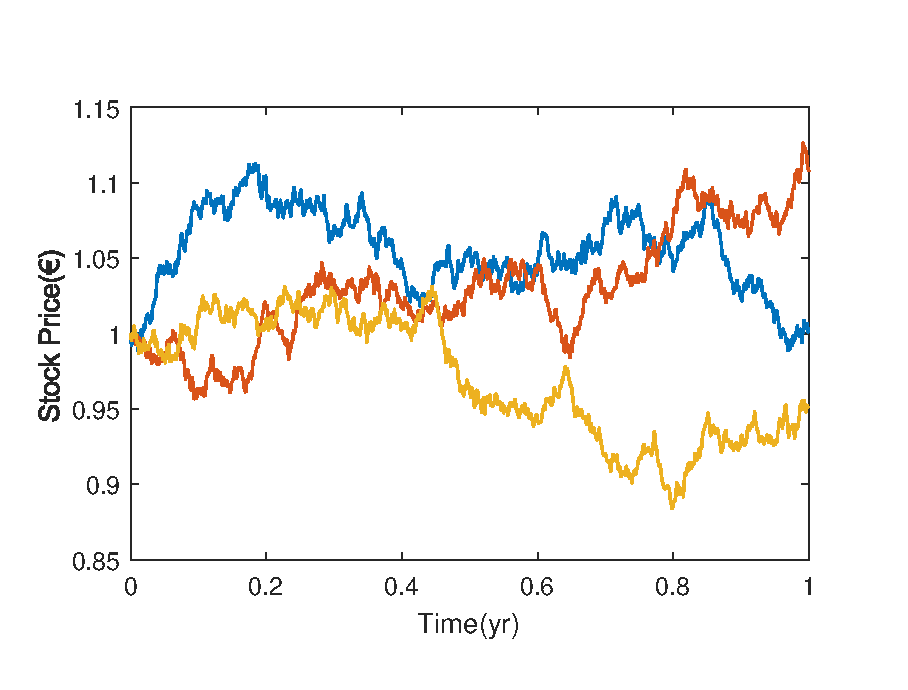
\includegraphics[width=0.9\columnwidth]{GBM.eps}
      \caption{Example of three GBM processes, using the parameters $r=\SI{0.06}{\per\year}$, $\sigma=0.05$, $S(0)=\SI{1}[\EUR]{}$ and time steps $\Delta t=10^{-3}\SI{}{\year}$.}\label{fig:GBM}
    \end{figure}
    
By simulating a large number of paths, some underlying tendencies might become apparent, which will prove useful in option pricing.


 American options, however, pose a much greater challenge.  Unlike European options, no analytic pricing model currently exists for this type of derivatives. Several numerical models have been proposed in the past in an attempt to solve this problem~\cite{Wilmott1,Hull}, such as the Longstaff-Schwartz algorithm~\citep{Longstaff}, which we shall approach in later sections of the present thesis.
\fi 

 
 
 
\section{Model Calibration}
\label{section:Model Calibration}
Both SABR and Heston stochastic volatility models contain variables that need to be calibrated in order to appropriately replicate market option prices.


Calibrating the models' parameters means finding the optimal values for these parameters such that the difference between the prices of market options and options priced under the models' assumptions is minimized. This difference should be measured with a cost function such as
\begin{equation}\label{cost}
\mathrm{Cost}(\theta)=\sum_{i=1}^n\sum_{j=1}^m\left(\frac{C_{\mathrm{market}}(T_i,K_j)-C_{\mathrm{model}}(\theta,T_i,K_j)}{C_{\mathrm{market}}(T_i,K_j)}\right)^2,
\end{equation}
\noindent where we denote $\theta$ as the model's parameter set and $C_{\mathrm{model}}(\cdot)$ and $C_{\mathrm{market}}(\cdot)$ correspond to the model and market option prices, respectively, for maturities $T_i,(i=1,\ldots,n)$ and strikes $K_j,(j=1,\ldots,m)$.

To obtain the value of the cost function for a given set of parameters, we need to calculate $m\times n$ model option prices. We could achieve this by applying the Monte Carlo method along with the discretization procedures described before.
Because we want to calibrate the model's parameters, a large number of instances of the cost function will have to be called for our optimization algorithms to converge to an optimal solution.
Thus, it can be seen that a very great number of Monte Carlo pricers will have to be executed. Even with GPU implementation and expensive hardware, using Monte Carlo to calibrate the model's parameters will become prohibitively slow. Furthermore, the Monte Carlo method is very noisy (i.e. two Monte Carlo pricers with the same initial conditions will produce slightly different outputs), making the whole convergence even more difficult.
An algorithm that takes several hours to converge does not meet market demands.

\hl{replace "Monte Carlo" by "MC"?}

The main reason why Heston and SABR models are so popular is the fact that both of them have closed-form solutions, shown in eqs. \eqref{CH}, \eqref{sabr} and \eqref{dynsabr}, that we can use to directly price the options under each model's assumptions, without the need to run the slow Monte Carlo pricer. The optimization algorithms should then converge much faster to the optimal solution for the model's parameters.






\subsection{Optimization Algorithms}
There are several possible algorithms to find the minimum value for the cost function shown in eq.\eqref{cost}.
Our main concern when choosing the best algorithms for calibration is the nonlinearity of the cost function. This is problematic because several local minima might exist and an inappropriate algorithm may get stuck in these points, causing the globally optimal solution to not be found.

With this issue in mind, we selected two powerful algorithms known as \emph{Multi-Start}~\cite{Ugray} and \emph{CMA-ES}~\cite{Hansen2} (short for Covariance Matrix Adaptation Evolution Strategy), which we will summarize below. It should be noted that we will only provide a general idea of how each optimizer works. For detailed descriptions, the original sources should be consulted.

\hl{how to deal with parameter boundaries? (All these algorithms enable the use of bounds which are required for our model parameters (e.g. the correlation parameter, $\rho$, in both Heston and SABR is obviously contained between $-1$ and $1$). Furthermore, they all require an initial guess at the values of the parameters, $\theta_0$, from which they will try to converge.)}

\subsubsection{Multi-Start Optimizer}
The Multi-Start optimizer is actually a combination of multiple simpler optimizers.
The algorithm starts by generating a set of different starting points. These points can be generated at random (i.e. by sampling from a uniform distribution) or using some complex meta-heuristic such as scatter search~\cite{Ugray}.

The algorithm then applies a simple optimizer to each of these starting points, finding a (local) minimum for all of them. Examples of such simple optimizers are the \emph{Active Set Method}, \emph{Sequential Quadratic Programming}, among others. We call these optimizers simple because they are only expected to converge to the (local) optimum closest to their starting point though at a very fast rate.

After local minima are found for all the selected starting points, the point where the cost function is minimized is chosen as optimal solution.

This procedure is depicted in Algorithm \ref{MSOpt}.

\begin{algorithm}[H]\label{MSOpt}
\DontPrintSemicolon
Generate $\theta_{0,i},\ \ i=1,\ldots,N$\tcc*[r]{Multiple starting points}
 \For{$i=1,\ldots,N$}{
  Run simple optimization algorithm with initial guess $\theta_{0,i}$\;
  Calculate $\mathrm{Cost}(\theta_i')$ for the obtained minimum $\theta_i'$\;
 }
 Optimal parameters: $\theta^{*}=\underset{\theta_i'}{\arg\min}\left\{\mathrm{Cost}(\theta_i')\right\}$\;
 \caption{Multi-Start Optimizer}
\end{algorithm}
\ 

One of the advantages of this algorithm is the fact that, because each simple algorithm execution is independent of the others (assuming no meta-heuristics are used), we can perform them in parallel, further increasing convergence speed.
As a disadvantage, we can point out the fact that, for functions with too many local minima, a large number of simple algorithm runs may be required, decreasing the calibration speed.

\hl{this function is in MATLAB}

\subsubsection{CMA-ES Optimizer}
The CMA-ES optimizer belongs to the class of evolutionary algorithms. These methods are based on the principle of biological evolution: at each iteration of the algorithm (generation), new candidate solutions (individuals) are generated from a given random distribution (mutation) obtained using the data of the previous solutions (parents). Of these newly generated solutions (individuals), we select the ones where the cost function is minimized (with the best fitness) to generate the candidate solutions of the next iterations (become parents of the next generations) and reject the others.

As for the CMA-ES in particular, the algorithm iteratively generates a multivariate normal distribution, modifying its mean and covariance matrix at each step.

We start with a $D$-dimensional normal distribution, centered around an initial guess $\theta^{(0)}$ (obtained \textit{a priori}), with a unit covariance matrix $C$ (i.e. $C=I$, the identity matrix), where $D$ denotes the number of variables of the selected model.

We then take $M$ samples from this distribution: $\theta^{(1)}_i\ i=1,\ldots,M$, which will be our first candidate solutions. We calculate the cost function for all of these points and rank them from best to worst. We keep only the $N$ best points (i.e. with the lowest cost) and discard the others.

A new normal distribution is then created. Its mean is calculated from a weighted average of the remaining $N$ points, with each weight inversely proportional to the point's cost. The covariance matrix is also generated from the remaining weighted $N$ points. However, to produce a faster convergence, the matrices from previous iterations are used additionally, i.e. we give some weight to the matrix generated from the selected points but we grant also weight to the previous matrices, assigning more weight to the most recent.

The previous steps are repeated for a number of iterations.

\hl{this algorithm finds the global optimum}

\hl{empirical rules to choose M, N, etc for CMA-ES}


\hl{citar Dilao} \cite{DilaoCMA}





\iffalse
\subsubsection{Polling Optimizer}
This powerful optimizer uses an adaptive mesh to find the minimum value of a function.
The algorithm starts at the provided initial guess $\theta_0=\left[\theta_{0,1},\ldots,\theta_{0,D}\right]$, where $D$ corresponds to the number of parameters. The cost function, $\mathrm{Cost}(\theta_0)$, is calculated for this point.

The algorithm then proceeds to generate $2D$ new points in the neighborhood of this initial point, where a displacement $\Delta\theta_i$ is added/subtracted to the initial point
\begin{equation}
\theta'_{i,\pm}=\theta_0\pm\left[0,\ldots,\Delta\theta_i,\ldots,0\right],\ \ \ i=1,\ldots,D,
\end{equation}
\noindent where, for simplicity, $\theta'_{i,\pm}$ denotes both $\theta'_{i,+}$ and $\theta'_{i,-}$.

The cost function is calculated for all these new points, $\mathrm{Cost}(\theta'_{i,\pm})$. If any of them have a lower cost than the original point, $\mathrm{Cost}(\theta_0)$, the point with the lowest cost function is accepted and the polling restarts i.e. we generate again $2D$ new points centered around this optimal point.

We repeat the previous step until all the $2D$ generated points present a higher cost function. When this happens, the displacement is reduced to half its value, $\Delta\theta_i/2$ and we restart the polling procedure for the optimal point found before.

The optimization stops when the cost of any of the generated points decreases past a threshold.

This method is systematized in Algorithm \ref{PolOpt}.

\begin{algorithm}[H]\label{PolOpt}
\DontPrintSemicolon
 Define $\theta=\theta_0=\left[\theta_{0,1},\ldots,\theta_{0,D}\right]$\tcc*[r]{Initial guess}
 \While{$\mathrm{Cost}(\theta)>\mathrm{Threshold}$}{
 Calculate $\mathrm{Cost}(\theta)$\;
 \For{i=1,\ldots,D}{ 
 Generate $\theta_{i,\pm}=\theta\pm\left[0,\ldots,\Delta\theta_i,\ldots,0\right]$\;
 Calculate $\mathrm{Cost}(\theta_{i,\pm})$\;
 }
 \eIf{$\mathrm{Cost}(\theta_{i,\pm})<\mathrm{Cost}(\theta),\ \ \forall\theta_{i,\pm}$}
 {$\theta=\underset{\theta_{i,\pm}}{\arg\min}\left\{\mathrm{Cost}(\theta_{i,\pm})\right\}$}
 {$\Delta\theta_i=\Delta\theta_i/2$}
 }
 Optimal parameters: $\theta^{*}=\theta$\;
 \caption{Deterministic Optimizer}
\end{algorithm}
\ 



In general, most procedures require some initial guess at the parameters' optimal values, $\theta_0$. The cost function for these values, $\mathrm{Cost}(\theta)$, is calculated. A new parameter vector, $\theta'$, is then generated in the neighborhood of the starting point and the cost function is recalculated, $\mathrm{Cost}(\theta')$. If the error decreases with this new vector (i.e. $\mathrm{Cost}(\theta')<\mathrm{Cost}(\theta)$), the new parameter values are assumed - otherwise they are discarded. This procedure is repeated until the cost function decreases below a threshold.
This algorithm is called deterministic because if we run the optimization twice with the same initial guess, the minima found in both instances will be the same.






%Two possible alternative optimizers exist to avoid this problem, which we will refer to as \emph{multi-start optimizer} and \emph{stochastic optimizer}.




\subsubsection{Simulated Annealing Optimizer}
As for the simulated annealing optimizer, the algorithm  starts with the initial guess, $\theta_0$, and calculates its cost function $\mathrm{Cost}(\theta)$. A new vector, $theta'$, is picked in the neighborhood of the first and its cost function, $\mathrm{Cost}(\theta')$, is calculated. 
There is a chance, defined by an acceptance probability function $P(\mathrm{Cost}(\theta),\mathrm{Cost}(\theta'))$, that the new vector is accepted, even if the cost function increases.
If this chance does not occur, the algorithm remains in the same point. 

The advantage of this optimizer is the fact that if the algorithm gets stuck at a local minimum, it may be able to escape from it until, ideally, the global optimum is found. An appropriate acceptance probability function must be found for the optimization.

This method is represented in Algorithm \ref{StochOpt}.

\begin{algorithm}[H]\label{StochOpt}
\DontPrintSemicolon
 Define $\theta=\theta_0$\tcc*[r]{Initial guess}
 \While{$\mathrm{Cost}(\theta)>\mathrm{Threshold}$}{
 Generate $\theta'$\tcc*[r]{New parameter vector}
  \If(\tcc*[f]{Acceptance Probability Function}){$P(\mathrm{Cost}(\theta),\mathrm{Cost}(\theta'))<\mathrm{random}(0,1)$}{Set $\theta=\theta'$\;}  
 }
 Optimal parameters: $\theta^{*}=\theta$\;
 \caption{Stochastic Optimizer}
\end{algorithm}
\ 
\fi






 % file "Thesis_Implementation.tex"
\cleardoublepage

%\input{Thesis_new_file} % add new .tex files for new chapters
% \cleardoublepage

%\input{Thesis_new_file} % add new .tex files for new chapters
% \cleardoublepage

%\input{Thesis_new_file} % add new .tex files for new chapters
% \cleardoublepage

%%%%%%%%%%%%%%%%%%%%%%%%%%%%%%%%%%%%%%%%%%%%%%%%%%%%%%%%%%%%%%%%%%%%%%%%
%                                                                      %
%     File: Thesis_Results.tex                                         %
%     Tex Master: Thesis.tex                                           %
%                                                                      %
%     Author: Andre C. Marta                                           %
%     Last modified :  2 Jul 2015                                      %
%                                                                      %
%%%%%%%%%%%%%%%%%%%%%%%%%%%%%%%%%%%%%%%%%%%%%%%%%%%%%%%%%%%%%%%%%%%%%%%%

\chapter{Results}
\label{chapter:results}

\hl{show data and mention where it came from. confidentiality, etc} % file "Thesis_Results.tex"
\cleardoublepage

%%%%%%%%%%%%%%%%%%%%%%%%%%%%%%%%%%%%%%%%%%%%%%%%%%%%%%%%%%%%%%%%%%%%%%%%
%                                                                      %
%     File: Thesis_Conclusions.tex                                     %
%     Tex Master: Thesis.tex                                           %
%                                                                      %
%     Author: Andre C. Marta                                           %
%     Last modified :  2 Jul 2015                                      %
%                                                                      %
%%%%%%%%%%%%%%%%%%%%%%%%%%%%%%%%%%%%%%%%%%%%%%%%%%%%%%%%%%%%%%%%%%%%%%%%

\chapter{Conclusions}
\label{chapter:conclusions}
Implement importance sampling - this has been done for Heston (and can easily be adapted to SABR) in \cite{Stilger}

Implement antithetic paths

we tried several algorithms but CMA and multi-start were better


use mean-reverting sabr

we could study the greeks % file "Thesis_Conclusions.tex"
\cleardoublepage

% ----------------------------------------------------------------------
%  Bibliography
% ----------------------------------------------------------------------

% Add entry in the table of contents as chapter
\phantomsection
\addcontentsline{toc}{chapter}{\bibname}

% Include all references in .bib file, even non-cited ones...
%\nocite{*} % this should be used carefully because it is not correct!

% Produces the bibliography section when processed by BibTeX
%
% Bibliography style
% > entries ordered alphabetically
%\bibliographystyle{plain}
% > unsorted with entries appearing in the order in which the citations appear.
%\bibliographystyle{unsrt}
% > entries ordered alphabetically, with first names and names of journals and months abbreviated
%\bibliographystyle{abbrv}
% > entries ordered alphabetically, with reference markers based on authors' initials and publication year
%\bibliographystyle{alpha}
%
% Replacement bibliography styles provided by 'natbib' package
% (plainnat.bst, abbrvnat.bst, unsrtnat.bst )
% > entries ordered alphabetically
%\bibliographystyle{plainnat}
% > unsorted with entries appearing in the order in which the citations appear.
%\bibliographystyle{unsrtnat}
% > entries ordered alphabetically, with first names and names of journals and months abbreviated
%\bibliographystyle{abbrvnat} % <<<<< SELECT IF USING REFERENCES BY AUTHOR/YEAR
% > entries ordered alphabetically, with reference markers based on authors' initials and publication year
%\bibliographystyle{alpha}
%
% Custom bibliography style adapted from 'natbib' package
%   (based on http://tex.stackexchange.com/questions/5053/is-it-possible-to-get-unsrt-abbrv-bibliography)
%   (unsrtnat.bst + abbrvnat.bst -> abbrvunsrtnat.bst)
%   (original files copied from:
%   http://tug.ctan.org/macros/latex/contrib/natbib/abbrvnat.bst
%   http://tug.ctan.org/macros/latex/contrib/natbib/unsrtnat.bst
% > unsorted with entries appearing in the order in which the citations appear, with first names and names of journals and months abbreviated.
\bibliographystyle{abbrvunsrtnat} % <<<<< SELECT IF USING REFERENCES BY NUMBER (CITATION ORDER)

% External bibliography database file in the BibTeX format
\bibliography{Thesis_bib_DB} % file "Thesis_bib_DB.bib"

\cleardoublepage

% ----------------------------------------------------------------------
%  Appendix (optional)
%
%  CAUTION: 1) the main document (up to the conclusions) shall not exceed 80 pages
%           2) the document shall not exceed a total of 100 pages (per IST regulations)
% ----------------------------------------------------------------------
\appendix

% add page number prefix according to apendix chapter (optional)
%\renewcommand{\thepage}{\thechapter.\arabic{page}}

% re-set arabic numbering (A.1,A.2,...) (optional, use only if chapter prefix is added)
%\setcounter{page}{1}

%%%%%%%%%%%%%%%%%%%%%%%%%%%%%%%%%%%%%%%%%%%%%%%%%%%%%%%%%%%%%%%%%%%%%%%%
%                                                                      %
%     File: Thesis_Appendix_A.tex                                      %
%     Tex Master: Thesis.tex                                           %
%                                                                      %
%     Author: Andre C. Marta                                           %
%     Last modified :  2 Jul 2015                                      %
%                                                                      %
%%%%%%%%%%%%%%%%%%%%%%%%%%%%%%%%%%%%%%%%%%%%%%%%%%%%%%%%%%%%%%%%%%%%%%%%

\chapter{Dupire's Formula Derivation}
\label{chapter:dupireformuladerivation}
Here is presented a brief demonstration of Dupire's formula, as shown in eq. \eqref{dupire}.

In his article, Dupire begins by assuming that the stock price $S$ follows a dynamic transition probability density function $p(S(t),t,S'(t'),t')$. In other words, integrating this function would result in the probability of the stock price reaching a price $S'$ at a time $t'$ having started at $S$ at time $t$.

The present value of a call option, $C(S,t,K,T)$, can be deduced as its expected future payoff, discounted backwards in time, which results in
\begin{equation}
\begin{split}\label{deriv0}
C(K,T)=e^{-r(T-t)}\mathbb{E}\left[\max\left(S'-K,0\right)\right]&=e^{-r(T-t)}\int_0^\infty\max\left(S'-K,0\right)p(S,t,S',T)dS'\\
&=e^{-r(T-t)}\int_K^\infty(S'-K)p(S,t,S',T)dS'.
\end{split}
\end{equation}
Deriving this result once with respect to the strike price $K$, we obtain
\begin{equation}
\pdv{C}{K}=-e^{-r(T-t)}\int_K^\infty p(S,t,S',T)dS'.
\end{equation}
Deriving again with respect to the same variable results in
\begin{equation}
\pdv{^2C}{K^2}=e^{-r(T-t)}p(S,t,S',T).
\end{equation}

Due to its stochastic nature, the transition probability density function follows the Fokker-Planck equation, given by
\begin{equation}\label{FokkerPlanck}
\pdv{p}{T}=\frac{1}{2}\sigma^2\pdv{^2(S^2p)}{S^2}-r\pdv{(Sp)}{S}.
\end{equation}
\noindent with $\sigma$ our, still unknown, function of $S$ and $t$, evaluated at $t=T$.

From eq. \ref{deriv0} we can easily derive
\begin{equation}
\pdv{C}{T}=-rC+e^{-r(T-t)}\int_K^\infty(S'-K)\pdv{p}{T}dS'.
\end{equation}
Using eq. \ref{FokkerPlanck}, we can transform this relation into
\begin{equation}
\pdv{C}{T}=-rC+e^{-r(T-t)}\int_K^\infty(S'-K)\left(\frac{1}{2}\sigma^2\pdv{^2(S'^2p)}{S'^2}-r\pdv{(S'p)}{S'}\right)dS'.
\end{equation}
Integrating twice by parts and collecting all terms, we get
\begin{equation}
\pdv{C}{T}=\frac{1}{2}\sigma^2K^2\pdv{^2C}{K^2}-rK\pdv{C}{K}.
\end{equation}
Rearranging all terms, we are left with the Dupire's formula
\begin{equation}
\sigma=\sqrt{\frac{\displaystyle\pdv{C}{T}+rK\pdv{C}{K}}{\displaystyle\frac{1}{2}K^2\pdv{^2C}{K^2}}}.
\end{equation}



 % file "Thesis_Appendix_A.tex"
\cleardoublepage


%%%%%%%%%%%%%%%%%%%%%%%%%%%%%%%%%%%%%%%%%%%%%%%%%%%%%%%%%%%%%%%%%%%%%%%%%
%                                                                      %
%     File: Thesis_Appendix_B.tex                                      %
%     Tex Master: Thesis.tex                                           %
%                                                                      %
%     Author: Andre C. Marta                                           %
%     Last modified :  2 Jul 2015                                      %
%                                                                      %
%%%%%%%%%%%%%%%%%%%%%%%%%%%%%%%%%%%%%%%%%%%%%%%%%%%%%%%%%%%%%%%%%%%%%%%%

\chapter{CMA-ES Algorithm Formulas}
\label{chapter:CMAESAlg}

Here we present the formulas required for the calculation of the mean vector, $\mathbf{m}$, and the covariance matrix, $\mathbf{C}$, to be used, at each iteration of the CMA-ES optimization algorithm, on the multivariate normal distribution
\begin{equation}
N(\mathbf{x;m,C})=\frac{1}{\sqrt{(2\pi)^D|\mathrm{det}\mathbf{C}|}}\mathrm{exp}\left(-\frac{1}{2}(\mathbf{x}-\mathbf{m})^T\mathbf{C}^{-1}(\mathbf{x}-\mathbf{m})\right).
\end{equation}

\section{The Optimization Algorithm}
\subsection{Initialization}
We initialize the algorithm by setting the first mean vector, $\mathbf{m}^{(0)}$, to some initial guess, $\theta_0$, and the covariance matrix to the unit matrix, $\mathbf{C}^{(0)}=\mathbf{I}$.

\subsection{Sampling}
We sample $\lambda$ points, $\mathbf{y}_i^{(1)},\ i=1,\ldots,\lambda$, from a multivariate normal distribution $N(\mathbf{x};\mathbf{0},\mathbf{C}^{(0)})$, generating the first candidate solutions
\begin{equation}
\mathbf{x}^{(1)}_i=\mathbf{m}^{(0)}+\sigma^{(0)}\mathbf{y}^{(1)}_i, \ \ \ \ \ i=1,\ldots,\lambda,
\end{equation} 
\noindent where $\sigma^{(0)}=1$.

\subsection{Classification}
The candidate solutions are ordered based on their cost function, such that we denote $\mathbf{x}^{(1)}_{i:\lambda}$ as the $i$-th best classified point from the set $\mathbf{x}^{(1)}_1,\ldots,\mathbf{x}^{(1)}_\lambda$. In other words, $\mathrm{Cost}(\mathbf{x}_{1:\lambda}^{(1)})\leq \mathrm{Cost}(\mathbf{x}_{2:\lambda}^{(1)})\leq\ldots\leq \mathrm{Cost}(\mathbf{x}_{\lambda:\lambda}^{(1)})$.

\subsection{Selection}
From the ordered set $\mathbf{x}^{(1)}_{i:\lambda}$ we choose the first $\mu$ data points (with the lowest cost) and discard the others.
We then define the weights $\omega_i$ as
\begin{equation}
\omega_i=\frac{\left(\log\left(\mu+1/2\right)-\log(i)\right)}{\sum_{i=1}^\mu\left(\log\left(\mu+1/2\right)-\log(i)\right)}, \ \ \ \ \ i=1,\ldots,\mu.
\end{equation}

As an alternative we could also use $\omega_i=1/\mu$.


\subsection{Adaptation}
We are finally able to calculate the new mean vector and covariance matrix using
\begin{equation}
\left\langle\mathbf{y}^{(k)}\right\rangle_w=\sum_{i=1}^\mu\omega_i\mathbf{y}^{(k)}_{i:\lambda},
\end{equation}
\begin{equation}\label{mean}
\mathbf{m}^{(k)}=\mathbf{m}^{(k-1)}+\sigma^{(k-1)}\left\langle\mathbf{y}^{(k)}\right\rangle_w=\sum_{i=1}^\mu\omega_i\mathbf{x}^{(k)}_{i:\lambda},
\end{equation}
\begin{equation}
\mathbf{p}^{(k)}_\sigma=(1-c_\sigma)\mathbf{p}^{(k-1)}_\sigma+\sqrt{c_\sigma(2-c_\sigma)\mu_{\mathrm{eff}}}\left(\mathbf{C}^{(k-1)}\right)^{-1/2}\left\langle\mathbf{y}^{(k)}\right\rangle_w,
\end{equation}
\begin{equation}
\sigma^{(k)}=\sigma^{(k-1)}\mathrm{exp}\left(\frac{c_\sigma}{d_\sigma}\left(\frac{\|\mathbf{p}^{(k)}_\sigma\|}{E^*}-1\right)\right),
\end{equation}
\begin{equation}
\mathbf{p}^{(k)}_c=(1-c_c)\mathbf{p}^{(k-1)}_c+h_\sigma^{(k)}\sqrt{c_c(2-c_c)\mu_{\mathrm{eff}}}\left\langle\mathbf{y}^{(k)}\right\rangle_w,
\end{equation}
\begin{equation}\label{covariance}
\mathbf{C}^{(k)}=\left(1-c_1-c_\mu\right)\mathbf{C}^{(k-1)}+c_1\left(\mathbf{p}_c^{(k)}\left(\mathbf{p}_c^{(k)}\right)^T+\delta\left(h_\sigma^{(k)}\right)\mathbf{C}^{(k-1)}\right)+c_\mu\sum_{i=1}^\mu\omega_i\mathbf{y}^{(k)}_{i:\lambda}\left(\mathbf{y}^{(k)}_{i:\lambda}\right)^T,
\end{equation}
\noindent where we define
\begin{equation}
\mu_{\mathrm{eff}}=\left(\sum_{i=1}^\mu\omega_i^2\right)^{-1},
\end{equation}
\begin{equation}
c_c=\frac{4+\mu_{\mathrm{eff}}/D}{D+4+2\mu_{\mathrm{eff}}/D},
\end{equation}
\begin{equation}
c_\sigma=\frac{\mu_{\mathrm{eff}}+2}{D+\mu_{\mathrm{eff}}+5},
\end{equation}
\begin{equation}
d_\sigma=1+2\max\left(0,\ \sqrt{\frac{\mu_{\mathrm{eff}}-1}{D+1}}-1\right)+c_\sigma,
\end{equation}
\begin{equation}
c_1=\frac{2}{(D+1.3)^2+\mu_{\mathrm{eff}}},
\end{equation}
\begin{equation}
c_\mu=\min\left(1-c_1,\ 2\frac{\mu_{\mathrm{eff}}-2+1/\mu_{\mathrm{eff}}}{(D+2)^2+\mu_{\mathrm{eff}}}\right),
\end{equation}
\begin{equation}
E^*=\frac{\sqrt{2}\Gamma\left(\frac{D+1}{2}\right)}{\Gamma\left(\frac{D}{2}\right)},
\end{equation}
\begin{equation}h_\sigma^{(k)}=
\begin{cases} 
      1, & \mathrm{if} \frac{\|\mathbf{p}^{(k)}_\sigma\|}{\sqrt{1-\left(1-c_\sigma\right)^{2(k+1)}}}<\left(1.4+\frac{2}{D+1}\right)E^*\\
      0, & \mathrm{otherwise}
   \end{cases},
\end{equation}
\begin{equation}
\delta\left(h_\sigma^{(k)}\right)=\left(1-h_\sigma^{(k)}\right)c_c\left(2-c_c\right),
\end{equation}
\begin{equation}
\left(\mathbf{C}^{(k)}\right)^{-1/2}=\mathbf{B}\left(\mathbf{D}^{(k)}\right)^{-1}\mathbf{B}^T,
\end{equation}
\noindent with $D$ corresponding to the number of parameters of the model (i.e. the dimensions of the sample space) and we define $\mathbf{p}_\sigma^{(0)}=\mathbf{p}_c^{(0)}=0$.


This steps are iterated until the termination criterion is met.












 % file "Thesis_Appendix_A.tex"
%\cleardoublepage

%%%%%%%%%%%%%%%%%%%%%%%%%%%%%%%%%%%%%%%%%%%%%%%%%%%%%%%%%%%%%%%%%%%%%%%%
%                                                                      %
%     File: Thesis_Appendix_B.tex                                      %
%     Tex Master: Thesis.tex                                           %
%                                                                      %
%     Author: Andre C. Marta                                           %
%     Last modified :  2 Jul 2015                                      %
%                                                                      %
%%%%%%%%%%%%%%%%%%%%%%%%%%%%%%%%%%%%%%%%%%%%%%%%%%%%%%%%%%%%%%%%%%%%%%%%

\chapter{CMA-ES Algorithm Formulas}
\label{chapter:CMAESAlg}

Here we present the formulas required for the calculation of the mean vector, $\mathbf{m}$, and the covariance matrix, $\mathbf{C}$, to be used, at each iteration of the CMA-ES optimization algorithm, on the multivariate normal distribution
\begin{equation}
N(\mathbf{x;m,C})=\frac{1}{\sqrt{(2\pi)^D|\mathrm{det}\mathbf{C}|}}\mathrm{exp}\left(-\frac{1}{2}(\mathbf{x}-\mathbf{m})^T\mathbf{C}^{-1}(\mathbf{x}-\mathbf{m})\right).
\end{equation}

We will directly follow the steps shown in \citep{DilaoCMA}. For a more in-depth explanation of the algorithm, refer to the cited article.

\section{The Optimization Algorithm}
\subsection{Initialization}
We initialize the algorithm by setting the first mean vector, $\mathbf{m}^{(0)}$, to some initial guess, $\theta_0$, and the covariance matrix to the unit matrix, $\mathbf{C}^{(0)}=\mathbf{I}$.

\subsection{Sampling}
We sample $\lambda$ points, $\mathbf{y}_i^{(1)},\ i=1,\ldots,\lambda$, from a multivariate normal distribution $N(\mathbf{x};\mathbf{0},\mathbf{C}^{(0)})$, generating the first candidate solutions
\begin{equation}
\mathbf{x}^{(1)}_i=\mathbf{m}^{(0)}+\sigma^{(0)}\mathbf{y}^{(1)}_i, \ \ \ \ \ i=1,\ldots,\lambda,
\end{equation} 
\noindent where $\sigma^{(0)}=1$.

\subsection{Classification}
The candidate solutions are ordered based on their cost function, such that we denote $\mathbf{x}^{(1)}_{i:\lambda}$ as the $i$-th best classified point from the set $\mathbf{x}^{(1)}_1,\ldots,\mathbf{x}^{(1)}_\lambda$. In other words, $\mathrm{Cost}(\mathbf{x}_{1:\lambda}^{(1)})\leq \mathrm{Cost}(\mathbf{x}_{2:\lambda}^{(1)})\leq\ldots\leq \mathrm{Cost}(\mathbf{x}_{\lambda:\lambda}^{(1)})$.

\subsection{Selection}
From the ordered set $\mathbf{x}^{(1)}_{i:\lambda}$ we choose the first $\mu$ data points (with the lowest cost) and discard the others.
We then define the weights $\omega_i$ as
\begin{equation}
\omega_i=\frac{\left(\log\left(\mu+1/2\right)-\log(i)\right)}{\sum_{i=1}^\mu\left(\log\left(\mu+1/2\right)-\log(i)\right)}, \ \ \ \ \ i=1,\ldots,\mu.
\end{equation}

As an alternative we could also use $\omega_i=1/\mu$.


\subsection{Adaptation}
We are finally able to calculate the new mean vector and covariance matrix using
\begin{equation}
\left\langle\mathbf{y}^{(k)}\right\rangle_w=\sum_{i=1}^\mu\omega_i\mathbf{y}^{(k)}_{i:\lambda},
\end{equation}
\begin{equation}\label{mean}
\mathbf{m}^{(k)}=\mathbf{m}^{(k-1)}+\sigma^{(k-1)}\left\langle\mathbf{y}^{(k)}\right\rangle_w=\sum_{i=1}^\mu\omega_i\mathbf{x}^{(k)}_{i:\lambda},
\end{equation}
\begin{equation}
\mathbf{p}^{(k)}_\sigma=(1-c_\sigma)\mathbf{p}^{(k-1)}_\sigma+\sqrt{c_\sigma(2-c_\sigma)\mu_{\mathrm{eff}}}\left(\mathbf{C}^{(k-1)}\right)^{-1/2}\left\langle\mathbf{y}^{(k)}\right\rangle_w,
\end{equation}
\begin{equation}
\sigma^{(k)}=\sigma^{(k-1)}\mathrm{exp}\left(\frac{c_\sigma}{d_\sigma}\left(\frac{\|\mathbf{p}^{(k)}_\sigma\|}{E^*}-1\right)\right),
\end{equation}
\begin{equation}
\mathbf{p}^{(k)}_c=(1-c_c)\mathbf{p}^{(k-1)}_c+h_\sigma^{(k)}\sqrt{c_c(2-c_c)\mu_{\mathrm{eff}}}\left\langle\mathbf{y}^{(k)}\right\rangle_w,
\end{equation}
\begin{equation}\label{covariance}
\mathbf{C}^{(k)}=\left(1-c_1-c_\mu\right)\mathbf{C}^{(k-1)}+c_1\left(\mathbf{p}_c^{(k)}\left(\mathbf{p}_c^{(k)}\right)^T+\delta\left(h_\sigma^{(k)}\right)\mathbf{C}^{(k-1)}\right)+c_\mu\sum_{i=1}^\mu\omega_i\mathbf{y}^{(k)}_{i:\lambda}\left(\mathbf{y}^{(k)}_{i:\lambda}\right)^T,
\end{equation}
\noindent where we define
\begin{equation}
\mu_{\mathrm{eff}}=\left(\sum_{i=1}^\mu\omega_i^2\right)^{-1},
\end{equation}
\begin{equation}
c_c=\frac{4+\mu_{\mathrm{eff}}/D}{D+4+2\mu_{\mathrm{eff}}/D},
\end{equation}
\begin{equation}
c_\sigma=\frac{\mu_{\mathrm{eff}}+2}{D+\mu_{\mathrm{eff}}+5},
\end{equation}
\begin{equation}
d_\sigma=1+2\max\left(0,\ \sqrt{\frac{\mu_{\mathrm{eff}}-1}{D+1}}-1\right)+c_\sigma,
\end{equation}
\begin{equation}
c_1=\frac{2}{(D+1.3)^2+\mu_{\mathrm{eff}}},
\end{equation}
\begin{equation}
c_\mu=\min\left(1-c_1,\ 2\frac{\mu_{\mathrm{eff}}-2+1/\mu_{\mathrm{eff}}}{(D+2)^2+\mu_{\mathrm{eff}}}\right),
\end{equation}
\begin{equation}
E^*=\frac{\sqrt{2}\Gamma\left(\frac{D+1}{2}\right)}{\Gamma\left(\frac{D}{2}\right)},
\end{equation}
\begin{equation}h_\sigma^{(k)}=
\begin{cases} 
      1, & \mathrm{if} \frac{\|\mathbf{p}^{(k)}_\sigma\|}{\sqrt{1-\left(1-c_\sigma\right)^{2(k+1)}}}<\left(1.4+\frac{2}{D+1}\right)E^*\\
      0, & \mathrm{otherwise}
   \end{cases},
\end{equation}
\begin{equation}
\delta\left(h_\sigma^{(k)}\right)=\left(1-h_\sigma^{(k)}\right)c_c\left(2-c_c\right),
\end{equation}
\begin{equation}
\left(\mathbf{C}^{(k)}\right)^{-1/2}=\mathbf{B}\left(\mathbf{D}^{(k)}\right)^{-1}\mathbf{B}^T,
\end{equation}
\noindent with $D$ corresponding to the number of parameters of the model (i.e. the dimensions of the sample space) and we define $\mathbf{p}_\sigma^{(0)}=\mathbf{p}_c^{(0)}=0$.


These steps are repeated until the termination criterion is met.












 % file "Thesis_Appendix_A.tex"
% re-set arabic numbering (B.1,B.2,...) (optional, use only if chapter prefix is added)
%\setcounter{page}{1}

%%%%%%%%%%%%%%%%%%%%%%%%%%%%%%%%%%%%%%%%%%%%%%%%%%%%%%%%%%%%%%%%%%%%%%%%%
%                                                                      %
%     File: Thesis_Appendix_B.tex                                      %
%     Tex Master: Thesis.tex                                           %
%                                                                      %
%     Author: Andre C. Marta                                           %
%     Last modified :  2 Jul 2015                                      %
%                                                                      %
%%%%%%%%%%%%%%%%%%%%%%%%%%%%%%%%%%%%%%%%%%%%%%%%%%%%%%%%%%%%%%%%%%%%%%%%

\chapter{CMA-ES Algorithm Formulas}
\label{chapter:CMAESAlg}

Here we present the formulas required for the calculation of the mean vector, $\mathbf{m}$, and the covariance matrix, $\mathbf{C}$, to be used, at each iteration of the CMA-ES optimization algorithm, on the multivariate normal distribution
\begin{equation}
N(\mathbf{x;m,C})=\frac{1}{\sqrt{(2\pi)^D|\mathrm{det}\mathbf{C}|}}\mathrm{exp}\left(-\frac{1}{2}(\mathbf{x}-\mathbf{m})^T\mathbf{C}^{-1}(\mathbf{x}-\mathbf{m})\right).
\end{equation}

\section{The Optimization Algorithm}
\subsection{Initialization}
We initialize the algorithm by setting the first mean vector, $\mathbf{m}^{(0)}$, to some initial guess, $\theta_0$, and the covariance matrix to the unit matrix, $\mathbf{C}^{(0)}=\mathbf{I}$.

\subsection{Sampling}
We sample $\lambda$ points, $\mathbf{y}_i^{(1)},\ i=1,\ldots,\lambda$, from a multivariate normal distribution $N(\mathbf{x};\mathbf{0},\mathbf{C}^{(0)})$, generating the first candidate solutions
\begin{equation}
\mathbf{x}^{(1)}_i=\mathbf{m}^{(0)}+\sigma^{(0)}\mathbf{y}^{(1)}_i, \ \ \ \ \ i=1,\ldots,\lambda,
\end{equation} 
\noindent where $\sigma^{(0)}=1$.

\subsection{Classification}
The candidate solutions are ordered based on their cost function, such that we denote $\mathbf{x}^{(1)}_{i:\lambda}$ as the $i$-th best classified point from the set $\mathbf{x}^{(1)}_1,\ldots,\mathbf{x}^{(1)}_\lambda$. In other words, $\mathrm{Cost}(\mathbf{x}_{1:\lambda}^{(1)})\leq \mathrm{Cost}(\mathbf{x}_{2:\lambda}^{(1)})\leq\ldots\leq \mathrm{Cost}(\mathbf{x}_{\lambda:\lambda}^{(1)})$.

\subsection{Selection}
From the ordered set $\mathbf{x}^{(1)}_{i:\lambda}$ we choose the first $\mu$ data points (with the lowest cost) and discard the others.
We then define the weights $\omega_i$ as
\begin{equation}
\omega_i=\frac{\left(\log\left(\mu+1/2\right)-\log(i)\right)}{\sum_{i=1}^\mu\left(\log\left(\mu+1/2\right)-\log(i)\right)}, \ \ \ \ \ i=1,\ldots,\mu.
\end{equation}

As an alternative we could also use $\omega_i=1/\mu$.


\subsection{Adaptation}
We are finally able to calculate the new mean vector and covariance matrix using
\begin{equation}
\left\langle\mathbf{y}^{(k)}\right\rangle_w=\sum_{i=1}^\mu\omega_i\mathbf{y}^{(k)}_{i:\lambda},
\end{equation}
\begin{equation}\label{mean}
\mathbf{m}^{(k)}=\mathbf{m}^{(k-1)}+\sigma^{(k-1)}\left\langle\mathbf{y}^{(k)}\right\rangle_w=\sum_{i=1}^\mu\omega_i\mathbf{x}^{(k)}_{i:\lambda},
\end{equation}
\begin{equation}
\mathbf{p}^{(k)}_\sigma=(1-c_\sigma)\mathbf{p}^{(k-1)}_\sigma+\sqrt{c_\sigma(2-c_\sigma)\mu_{\mathrm{eff}}}\left(\mathbf{C}^{(k-1)}\right)^{-1/2}\left\langle\mathbf{y}^{(k)}\right\rangle_w,
\end{equation}
\begin{equation}
\sigma^{(k)}=\sigma^{(k-1)}\mathrm{exp}\left(\frac{c_\sigma}{d_\sigma}\left(\frac{\|\mathbf{p}^{(k)}_\sigma\|}{E^*}-1\right)\right),
\end{equation}
\begin{equation}
\mathbf{p}^{(k)}_c=(1-c_c)\mathbf{p}^{(k-1)}_c+h_\sigma^{(k)}\sqrt{c_c(2-c_c)\mu_{\mathrm{eff}}}\left\langle\mathbf{y}^{(k)}\right\rangle_w,
\end{equation}
\begin{equation}\label{covariance}
\mathbf{C}^{(k)}=\left(1-c_1-c_\mu\right)\mathbf{C}^{(k-1)}+c_1\left(\mathbf{p}_c^{(k)}\left(\mathbf{p}_c^{(k)}\right)^T+\delta\left(h_\sigma^{(k)}\right)\mathbf{C}^{(k-1)}\right)+c_\mu\sum_{i=1}^\mu\omega_i\mathbf{y}^{(k)}_{i:\lambda}\left(\mathbf{y}^{(k)}_{i:\lambda}\right)^T,
\end{equation}
\noindent where we define
\begin{equation}
\mu_{\mathrm{eff}}=\left(\sum_{i=1}^\mu\omega_i^2\right)^{-1},
\end{equation}
\begin{equation}
c_c=\frac{4+\mu_{\mathrm{eff}}/D}{D+4+2\mu_{\mathrm{eff}}/D},
\end{equation}
\begin{equation}
c_\sigma=\frac{\mu_{\mathrm{eff}}+2}{D+\mu_{\mathrm{eff}}+5},
\end{equation}
\begin{equation}
d_\sigma=1+2\max\left(0,\ \sqrt{\frac{\mu_{\mathrm{eff}}-1}{D+1}}-1\right)+c_\sigma,
\end{equation}
\begin{equation}
c_1=\frac{2}{(D+1.3)^2+\mu_{\mathrm{eff}}},
\end{equation}
\begin{equation}
c_\mu=\min\left(1-c_1,\ 2\frac{\mu_{\mathrm{eff}}-2+1/\mu_{\mathrm{eff}}}{(D+2)^2+\mu_{\mathrm{eff}}}\right),
\end{equation}
\begin{equation}
E^*=\frac{\sqrt{2}\Gamma\left(\frac{D+1}{2}\right)}{\Gamma\left(\frac{D}{2}\right)},
\end{equation}
\begin{equation}h_\sigma^{(k)}=
\begin{cases} 
      1, & \mathrm{if} \frac{\|\mathbf{p}^{(k)}_\sigma\|}{\sqrt{1-\left(1-c_\sigma\right)^{2(k+1)}}}<\left(1.4+\frac{2}{D+1}\right)E^*\\
      0, & \mathrm{otherwise}
   \end{cases},
\end{equation}
\begin{equation}
\delta\left(h_\sigma^{(k)}\right)=\left(1-h_\sigma^{(k)}\right)c_c\left(2-c_c\right),
\end{equation}
\begin{equation}
\left(\mathbf{C}^{(k)}\right)^{-1/2}=\mathbf{B}\left(\mathbf{D}^{(k)}\right)^{-1}\mathbf{B}^T,
\end{equation}
\noindent with $D$ corresponding to the number of parameters of the model (i.e. the dimensions of the sample space) and we define $\mathbf{p}_\sigma^{(0)}=\mathbf{p}_c^{(0)}=0$.


This steps are iterated until the termination criterion is met.












 % file "Thesis_Appendix_B.tex"
%\cleardoublepage



\section{Topic Overview}
\label{section:overview}

Provide an overview of the topic to be studied...


\section{Objectives}
\label{section:objectives}

Explicitly state the objectives set to be achieved with this thesis...


\section{Thesis Outline}
\label{section:outline}

Briefly explain the contents of the different chapters...



\section{Theoretical Overview}
\label{section:teoroverview}


Some overview of the underlying theory about the topic...


%%%%%%%%%%%%%%%%%%%%%%%%%%%%%%%%%%%%%%%%%%%%%%%%%%%%%%%%%%%%%%%%%%%%%%%%
\section{Theoretical Model 1}
\label{section:theory1}



Multiple citations are compressed when using the {\tt sort\&compress} option when loading the {\tt natbib} package as {\tt \textbackslash usepackage[numbers,sort\&compress]\{natbib\}} in file {\tt Thesis\_Preamble.tex}, resulting in citations like ~\citep{Hull,Wilmott}.


%%%%%%%%%%%%%%%%%%%%%%%%%%%%%%%%%%%%%%%%%%%%%%%%%%%%%%%%%%%%%%%%%%%%%%%%
\section{Theoretical Model 2}
\label{section:theory2}

Other models...




Insert your chapter material here...

%%%%%%%%%%%%%%%%%%%%%%%%%%%%%%%%%%%%%%%%%%%%%%%%%%%%%%%%%%%%%%%%%%%%%%%%
\section{Numerical Model}
\label{section:model}

Description of the numerical implementation of the models explained in Chapter~\ref{chapter:background}...


%%%%%%%%%%%%%%%%%%%%%%%%%%%%%%%%%%%%%%%%%%%%%%%%%%%%%%%%%%%%%%%%%%%%%%%%
\section{Verification and Validation}
\label{section:verification}

Basic test cases to compare the implemented model against other numerical tools (verification) and experimental data (validation)...



Insert your chapter material here...


%%%%%%%%%%%%%%%%%%%%%%%%%%%%%%%%%%%%%%%%%%%%%%%%%%%%%%%%%%%%%%%%%%%%%%%%
\section{Problem Description}
\label{section:problem}

Description of the baseline problem...


%%%%%%%%%%%%%%%%%%%%%%%%%%%%%%%%%%%%%%%%%%%%%%%%%%%%%%%%%%%%%%%%%%%%%%%%
\section{Baseline Solution}
\label{section:baseline}

Analysis of the baseline solution...


%%%%%%%%%%%%%%%%%%%%%%%%%%%%%%%%%%%%%%%%%%%%%%%%%%%%%%%%%%%%%%%%%%%%%%%%
\section{Enhanced Solution}
\label{section:enhanced}

Quest for the optimal solution...


% ----------------------------------------------------------------------
\subsection{Figures}
\label{subsection:figures}

Insert your section material and possibly a few figures...

Make sure all figures presented are referenced in the text!


% ----------------------------------------------------------------------
\subsubsection{Images}
\label{subsection:images}

\iffalse
\begin{figure}[!htb]
  \centering
  \includegraphics[width=0.25\textwidth]{Airbus_A350.jpg}
  \caption[Caption for figure in TOC.]{Caption for figure.}
  \label{fig:airbus1}
\end{figure}

\begin{figure}[!htb]
  \begin{subfigmatrix}{2}
    \subfigure[Airbus A320]{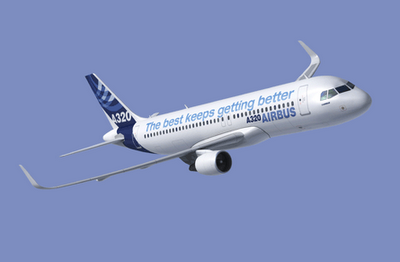
\includegraphics[width=0.49\linewidth]{Airbus_A320_sharklets.png}}
    \subfigure[Bombardier CRJ200]{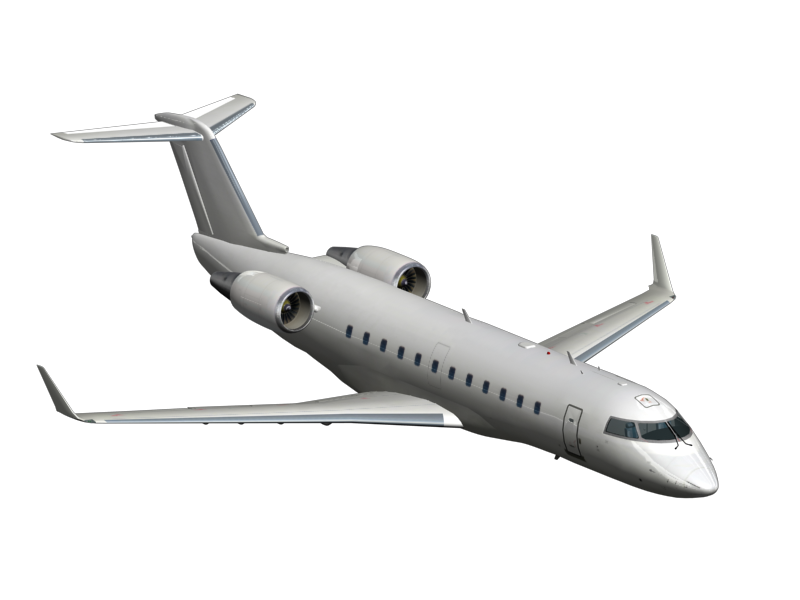
\includegraphics[width=0.49\linewidth]{Bombardier_CRJ200.png}}
  \end{subfigmatrix}
  \caption{Some aircrafts.}
  \label{fig:aircrafts}
\end{figure}
\fi

Make reference to Figures.

By default, the supported file types are {\it .png,.pdf,.jpg,.mps,.jpeg,.PNG,.PDF,.JPG,.JPEG}.

See \url{http://mactex-wiki.tug.org/wiki/index.php/Graphics_inclusion} for adding support to other extensions.


% ----------------------------------------------------------------------
\subsubsection{Drawings}
\label{subsection:drawings}

Insert your subsection material and for instance a few drawings...

The schematic illustrated in Fig.can represent some sort of algorithm.
\iffalse
\begin{figure}[!htb]
  \centering
  \scriptsize
%  \footnotesize 
%  \small
  \setlength{\unitlength}{0.9cm}
  \begin{picture}(8.5,6)
    \linethickness{0.3mm}

    \put(3,6){\vector(0,-1){1}}
    \put(3.5,5.4){$\bf \alpha$}
    \put(3,4.5){\oval(6,1){}}
    %\put(0,4){\framebox(6,1){}}
    \put(0.3,4.4){Grid Generation: \quad ${\bf x} = {\bf x}\left({\bf \alpha}\right)$}

    \put(3,4){\vector(0,-1){1}}
    \put(3.5,3.4){$\bf x$}
    \put(3,2.5){\oval(6,1){}}
    %\put(0,2){\framebox(6,1){}}
    \put(0.3,2.4){Flow Solver: \quad ${\cal R}\left({\bf x},{\bf q}\left({\bf x}\right)\right) = 0$}

    \put(6.0,2.5){\vector(1,0){1}}
    \put(6.4,3){$Y_1$}

    \put(3,2){\vector(0,-1){1}}
    \put(3.5,1.4){$\bf q$}
    \put(3,0.5){\oval(6,1){}}
    %\put(0,0){\framebox(6,1){}}
    \put(0.3,0.4){Structural Solver: \quad ${\cal M}\left({\bf x},{\bf q}\left({\bf x}\right)\right) = 0$}

    \put(6.0,0.5){\vector(1,0){1}}
    \put(6.4,1){$Y_2$}

    %\put(7.8,2.5){\oval(1.6,5){}}
    \put(7.0,0){\framebox(1.6,5){}}
    \put(7.1,2.5){Optimizer}
    \put(7.8,5){\line(0,1){1}}
    \put(7.8,6){\line(-1,0){4.8}}
  \end{picture}
  \caption{Schematic of some algorithm.}
  \label{fig:algorithm}
\end{figure}
\fi

% ----------------------------------------------------------------------
\subsection{Equations}
\label{subsection:equations}

Equations can be inserted in different ways.

The simplest way is in a separate line like this

\begin{equation}
  \frac{{\rm d} q_{ijk}}{{\rm d} t} + {\cal R}_{ijk}({\bf q}) = 0 \,.
\label{eq:ode}
\end{equation}

If the equation is to be embedded in the text. One can do it like this ${\partial {\cal R}}/{\partial {\bf q}}=0$.

It may also be split in different lines like this
\iffalse
\begin{eqnarray}
  {\rm Minimize}   && Y({\bf \alpha},{\bf q}({\bf \alpha}))            \nonumber           \\
  {\rm w.r.t.}     && {\bf \alpha} \,,                                 \label{eq:minimize} \\
  {\rm subject~to} && {\cal R}({\bf \alpha},{\bf q}({\bf \alpha})) = 0 \nonumber           \\
                   &&       C ({\bf \alpha},{\bf q}({\bf \alpha})) = 0 \,. \nonumber
\end{eqnarray}

It is also possible to use subequations. Equations~\ref{eq:continuity}, \ref{eq:momentum} and \ref{eq:energy} form the Naver--Stokes equations~\ref{eq:NavierStokes}.

\begin{subequations}
    \begin{equation}
    \frac{\partial \rho}{\partial t} + \frac{\partial}{\partial x_j}\left( \rho u_j \right) = 0 \,,
    \label{eq:continuity}
    \end{equation}
    \begin{equation}
    \frac{\partial}{\partial t}\left( \rho u_i \right) + \frac{\partial}{\partial x_j} \left( \rho u_i u_j + p \delta_{ij} - \tau_{ji} \right) = 0, \quad i=1,2,3 \,,
    \label{eq:momentum}
    \end{equation}
    \begin{equation}
        \frac{\partial}{\partial t}\left( \rho E \right) + \frac{\partial}{\partial x_j} \left( \rho E u_j + p u_j - u_i \tau_{ij} + q_j \right) = 0 \,.
    \label{eq:energy}
    \end{equation}
\label{eq:NavierStokes}%
\end{subequations}
\fi

% ----------------------------------------------------------------------
\subsection{Tables}
\label{section:tables}

Insert your subsection material and for instance a few tables...

Make sure all tables presented are referenced in the text!

Follow some guidelines when making tables:
\iffalse
\begin{itemize}
  \item Avoid vertical lines
  \item Avoid “boxing up” cells, usually 3 horizontal lines are enough: above, below, and after heading
  \item Avoid double horizontal lines
  \item Add enough space between rows
\end{itemize}

\begin{table}[!htb]
  \renewcommand{\arraystretch}{1.2} % more space between rows
  \centering
  \begin{tabular}{lccc}
    \toprule
    Model           & $C_L$ & $C_D$ & $C_{M y}$ \\
    \midrule
    Euler           & 0.083 & 0.021 & -0.110    \\
    Navier--Stokes  & 0.078 & 0.023 & -0.101    \\
    \bottomrule
  \end{tabular}
  \caption[Table caption shown in TOC.]{Table caption.}
  \label{tab:aeroCoeff}
\end{table}

Make reference to Table \ref{tab:aeroCoeff}.

Tables \ref{tab:memory} and \ref{tab:multipleColumns} are examples of tables with merging columns:

\begin{table}[!htb]
  \renewcommand{\arraystretch}{1.2} % more space between rows
  \centering
  \begin{tabular}[]{lrr}
    \toprule
                & \multicolumn{2}{c}{\underline{Virtual memory [MB]}} \\
                & Euler       & Navier--Stokes \\
    \midrule
      Wing only &  1,000      &    2,000       \\
      Aircraft  &  5,000      &   10,000       \\
      (ratio)   & $5.0\times$ & $5.0\times$    \\
    \bottomrule
  \end{tabular}
  \caption{Memory usage comparison (in MB).}
  \label{tab:memory}
\end{table}

\begin{table}[!htb]
  \centering
  \renewcommand{\arraystretch}{1.2} % more space between rows
  \begin{tabular}{@{}rrrrcrrr@{}} % remove space to the vertical edges @{}...@{}
    \toprule
      & \multicolumn{3}{c}{$w = 2$} & \phantom{abc} & \multicolumn{3}{c}{$w = 4$} \\
    \cmidrule{2-4}
    \cmidrule{6-8}
      & $t=0$ & $t=1$ & $t=2$ && $t=0$ & $t=1$ & $t=2$ \\
    \midrule
      $dir=1$
      \\
      $c$ &  0.07 &  0.16 &  0.29 &&  0.36 &  0.71 &   3.18 \\
      $c$ & -0.86 & 50.04 &  5.93 && -9.07 & 29.09 &  46.21 \\
      $c$ & 14.27 &-50.96 &-14.27 && 12.22 &-63.54 &-381.09 \\
      $dir=0$
      \\
      $c$ &  0.03 &  1.24 &  0.21 &&  0.35 & -0.27 &  2.14 \\
      $c$ &-17.90 &-37.11 &  8.85 &&-30.73 & -9.59 & -3.00 \\
      $c$ &105.55 & 23.11 &-94.73 &&100.24 & 41.27 &-25.73 \\
    \bottomrule
  \end{tabular}
  \caption{Another table caption.}
  \label{tab:multipleColumns}
\end{table}

An example with merging rows can be seen in Tab.\ref{tab:multipleRows}.

\begin{table}[!htb]
  \renewcommand{\arraystretch}{1.2} % more space between rows
  \centering
  \begin{tabular}{ccccc}
    \toprule
      \multirow{2}{*}{ABC} & \multicolumn{4}{c}{header} \\
      \cmidrule{2-5} & 1.1 & 2.2 & 3.3 & 4.4 \\
    \midrule
      \multirow{2}{*}{IJK} & \multicolumn{2}{c}{\multirow{2}{*}{group}} & 0.5 & 0.6 \\
      \cmidrule{4-5}       & \multicolumn{2}{c}{}                       & 0.7 & 1.2 \\
    \bottomrule
  \end{tabular}
  \caption{Yet another table caption.}
  \label{tab:multipleRows}
\end{table}

If the table has too many columns, it can be scaled to fit the text widht, as in Tab.\ref{tab:scale}.
\begin{table}[!htb]
  \renewcommand{\arraystretch}{1.2} % more space between rows
  \centering
  \resizebox*{\textwidth}{!}{%
    \begin{tabular}[]{lcccccccccc}
      \toprule
        Variable &  a  &  b  &  c  &  d  &  e  &  f  &  g  &  h  &  i  &  j  \\
      \midrule
        Test 1   &  10,000 &  20,000 &  30,000 &  40,000 &  50,000 &  60,000 &  70,000 &  80,000 &  90,000 & 100,000 \\
        Test 2   &  20,000 &  40,000 &  60,000 &  80,000 & 100,000 & 120,000 & 140,000 & 160,000 & 180,000 & 200,000 \\
      \bottomrule
    \end{tabular}
  }%
  \caption{Very wide table.}
  \label{tab:scale}%
\end{table}
\fi

% ----------------------------------------------------------------------
\subsection{Mixing}
\label{section:mixing}

If necessary, a figure and a table can be put side-by-side as in Fig.
\iffalse
\begin{figure}[!htb]
  \begin{minipage}[b]{0.60\linewidth}
    \centering
    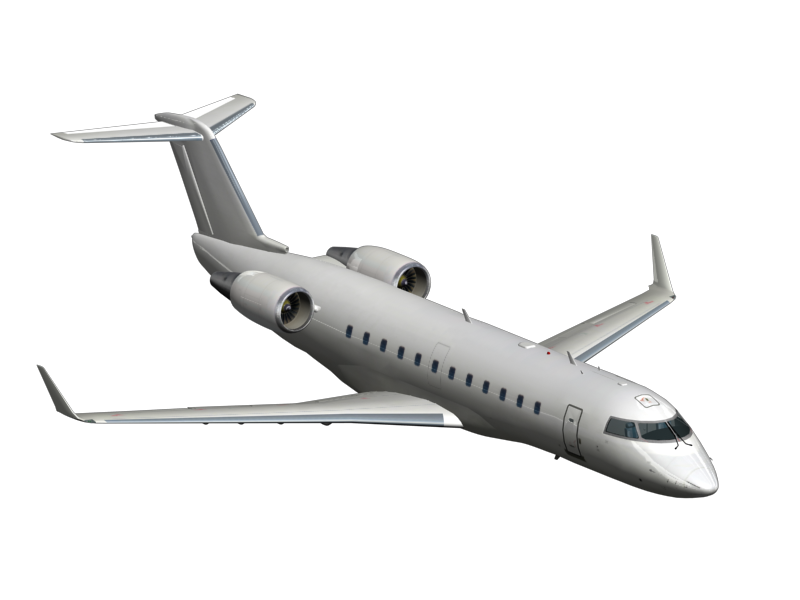
\includegraphics[width=\linewidth]{Bombardier_CRJ200}
  \end{minipage}%
  \begin{minipage}[b]{0.30\linewidth}
    \centering
    \begin{tabular}[b]{lll}
      \toprule
        \multicolumn{3}{c}{Legend} \\
      \midrule
        A & B & C \\
        0 & 0 & 0 \\
        0 & 1 & 0 \\
        1 & 0 & 0 \\
        1 & 1 & 1 \\
      \bottomrule
    \end{tabular}
    \vspace{5em}
  \end{minipage}
\caption{Figure and table side-by-side.}
\label{fig:side_by_side}
\end{figure}

\fi

Insert your chapter material here...


% ----------------------------------------------------------------------
\section{Achievements}
\label{section:achievements}

The major achievements of the present work...


% ----------------------------------------------------------------------
\section{Future Work}
\label{section:future}

A few ideas for future work...


% ----------------------------------------------------------------------
In case an appendix if deemed necessary, the document cannot exceed a total of 100 pages...

Some definitions and vector identities are listed in the section below.
\section{Vector identities}
\label{section:vectorIdentities}

\begin{equation}
	\nabla \times \left( \nabla \phi \right) = 0
	\label{eq:cross_nnp}
\end{equation}

\begin{equation}
	\nabla \cdot \left( \nabla \times {\bf u} \right) = 0
	\label{eq:dotCross_nnu}
\end{equation}
 % file "Template.tex"

% ----------------------------------------------------------------------
\end{document}
% ----------------------------------------------------------------------

